\documentclass{report}
\usepackage[T1]{fontenc} % Fontes T1
\usepackage[utf8]{inputenc} % Input UTF8
\usepackage[backend=biber, style=ieee]{biblatex} % para usar bibliografia
\usepackage{csquotes}
\usepackage[portuguese]{babel} %Usar língua portuguesa
\usepackage{blindtext} % Gerar texto automaticamente
\usepackage[printonlyused]{acronym}
\usepackage{hyperref} % para autoref
\usepackage{graphicx}
\usepackage{wrapfig}
\usepackage{caption}
\usepackage{subcaption}
\usepackage{multirow}
\usepackage{color}
\usepackage{xcolor}
\bibliography{bibliografia}


\begin{document}
%%
% Definições
%
\acrodefplural{vrm}[VRM's]{Voltage Regulator Modules}
\acrodefplural{gpu}[GPU's]{Graphics Processing Unit}
\acrodefplural{pg}[PG's]{Placas Gráficas}
\def\titulo{Placas Gráficas}
\def\data{\today}
\def\autores{Marco Almeida, Pedro Mendes}
\def\autorescontactos{(103440) marco.almeida@ua.pt, (103028) pmiguelsilvamendes@ua.pt}
\def\versao{Versão 1}
\def\departamento{Departamento de Eletrónica, Telecomunicações e Informática}
\def\empresa{Universidade de Aveiro}
\def\logotipo{ua.pdf}
%
%%%%%% CAPA %%%%%%
%
\renewcommand{\contentsname}{Índice}
\begin{titlepage}

\begin{center}
%
\vspace*{50mm}
%
{\Huge \titulo}\\ 
%
\vspace{10mm}
%
{\Large \empresa}\\
%
\vspace{10mm}
%
{\LARGE \autores}\\ 
%
\vspace{30mm}
%
\begin{figure}[h]
\center
\includegraphics{\logotipo}
\end{figure}
%
\vspace{30mm}
\end{center}
%
\begin{flushright}
\versao
\end{flushright}
\end{titlepage}

%%  Página de Título %%
\title{%
{\Huge\textbf{\titulo}}\\
{\Large \departamento\\ \empresa}
}
%
\author{%
    \autores \\
    \autorescontactos
}
%
\date{\data}
%
\maketitle

\pagenumbering{roman}

%%%%%% RESUMO %%%%%%
\begin{abstract}
Neste trabalho iremos aprofundar o tema de Placas Gráficas dedicadas, uma vez que achamos ser relevante para a cadeira de Laboratórios de Informática.

Para tal iremos estudar a história por detrás das Placas Gráficas e a sua demanda, o seu impacto tecnológico, os seus componentes, a sua evolução, grande parte da tecnologia que a rodeia e a \textit{scene} atual. 
\end{abstract}


\tableofcontents
\listoftables     % descomentar se necessário
\listoffigures    % descomentar se necessário


%%%%%%%%%%%%%%%%%%%%%%%%%%%%%%%
\clearpage
\pagenumbering{arabic}

%%%%%%%%%%%%%%%%%%%%%%%%%%%%%%%%
\chapter{O que são Placas Gráficas}
\label{gpu}
\section{Introdução}
\label{introduc}

As \acp{pg}, ou Placas de Vídeo, foram criadas com a finalidade de transformar a informação digital processada em uma imagem representada no monitor, sendo por isso responsável por todo o conteúdo visual e, consequentemente, necessária e presente em todos os computadores de forma a que possa ser transmitida uma imagem com a informação recolhida (salvo exceções de processadores com \ac{gpu} integrada).


\begin{figure}[h]
\centering
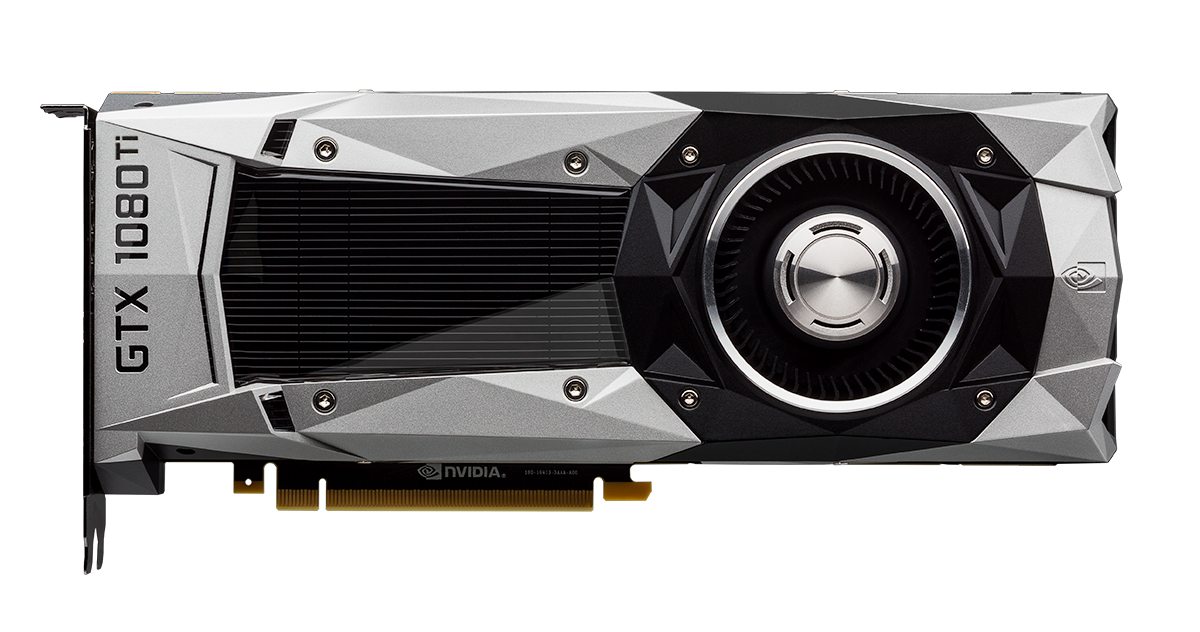
\includegraphics[width=0.5\textwidth]{1080ti.png}
\caption{Exemplo de Placa Gráfica}
\label{fig:1080ti}
\end{figure}

O uso das \acp{pg} varia conforme a função que for designada, podendo servir apenas para tarefas simples como trabalhar em programas básicos, visualizar fotografias ou vídeos, ou uma simples pesquisa na internet, até atividades que requerem um maior desempenho gráfico como em videojogos, programas de edição de imagem mais pesados, renderização 3D.
\clearpage
\section{Componentes e Respetivas Funções}
\label{comp}

As Placas de Vídeo possuem componentes (\autoref{fig:anatomia}), cada um com a sua função, que vão então ler a informação e transmiti-la ao utilizador e muito mais.

\begin{figure}[h]
\centering
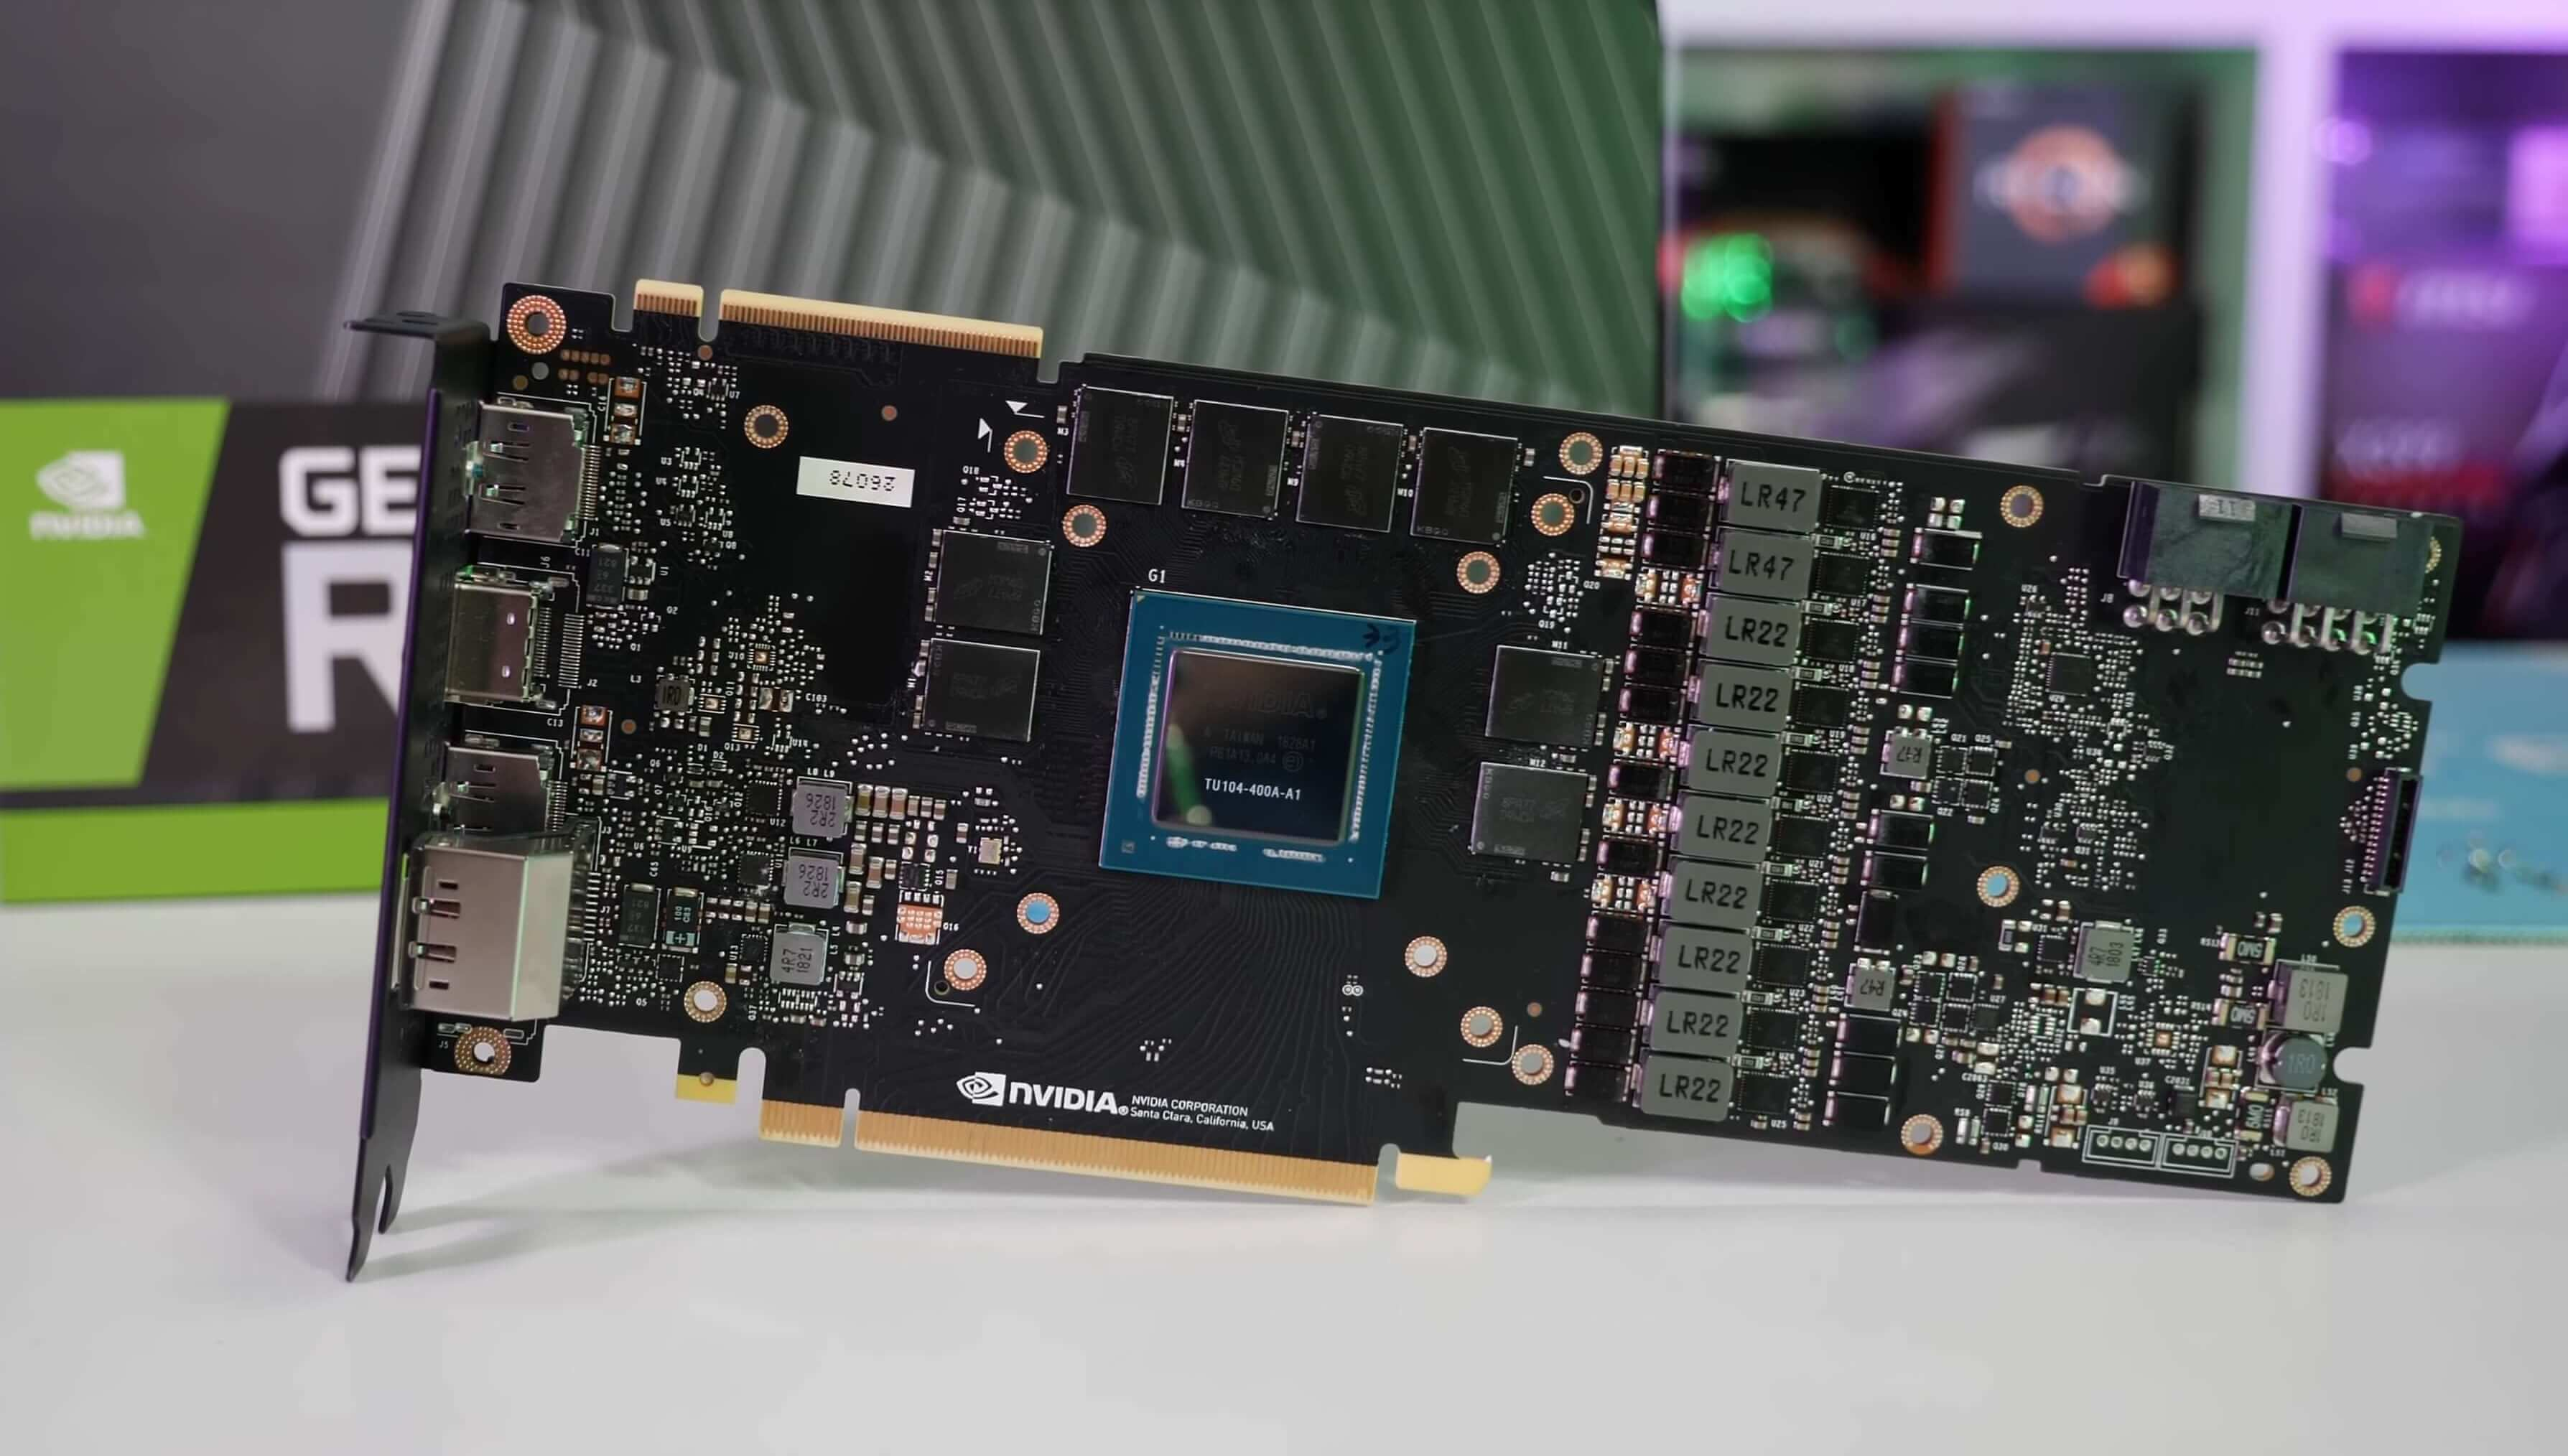
\includegraphics[width=1\textwidth]{anatomy.jpg}
\caption{A anatomia de uma placa gráfica}
\label{fig:anatomia}
\end{figure}

\clearpage
\subsection{GPU}
\label{sec.gpu}
A \ac{gpu} é o componente mais importante e o coração da placa gráfica, este componente faz todo o processamento na placa de vídeo. Geralmente, a maioria das placas gráficas possuem apenas um \ac{gpu} mas existem placas gráficas com mais do que um \ac{gpu}.

\begin{figure}[h]
\centering
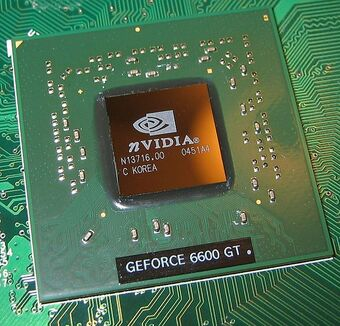
\includegraphics[width=0.4\textwidth]{gpunit.jpg}
\caption{Graphics Processing Unit}
\label{fig:gpu}
\end{figure}

A \ac{gpu} funciona de acordo com a sua arquitetura e esta varia de série para série e de fabricante para fabricante. Há milhares de \textit{cores} dentro das \acp{gpu} para processamento paralelo e \textit{multi-tasking} e estes \textit{cores} trabalham de forma diferente, dependendo da respetiva arquitetura.

São apelidados de \textit{CUDA Cores} pela \textit{Nvidia}\footnote{Nvidia Corporation, empresa multinacional fabricadora de placas de vídeo} e \textit{Stream Processors} pela \textit{AMD}\footnote{Advanced Micro Devices, Inc., empresa norte-americana fabricante de circuitos integrados, especialmente processadores e placas de vídeo}. 

Geralmente, quanto mais recente for a arquitetura (\autoref{tab:tab1}) da \ac{gpu}, mais performance e menos consumo de energia terá a placa de vídeo\cite{graphh}.

\begin{table}[h]
\begin{center}
\begin{tabular}{|c|c|c|c|l}
 \hline
 Fabricador & Arquitetura & GPU's & Data de Lançamento \\ [0.5ex] 
 \hline\hline
 AMD & Polaris & Série Radeon RX 500 & 2017\\ 
 \hline
 AMD & RDNA & Série RX 5000 &  2019\\
 \hline
 AMD & RDNA2 & Série RX 6000 & 2020\\
 \hline
 Nvidia & Pascal & Série GTX 1000 & 2016\\
 \hline
 Nvidia & Turing & Séries RTX 2000 & 2018\\ 
 \hline
 Nvidia & Ampere & Série RTX 3000 & 2020\\ [1ex] 
 \hline
\end{tabular}
\end{center}
\caption{As mais recentes arquiteturas de \acp{gpu}\label{tab:tab1}}
\end{table}
\clearpage
\subsubsection{Core Clock}

Para comparar \acp{pg}, recorre-se muitas vezes ao \textit{Core Clock}. O \textit{Core Clock} é a frequência a que opera o chip da Placa de Vídeo, a \ac{gpu}. Esta característica pode ser alterada pelo utilizador em pequenas quantidades utilizando software dedicado. (\autoref{fig:msi}).

\begin{figure}[h]
\centering
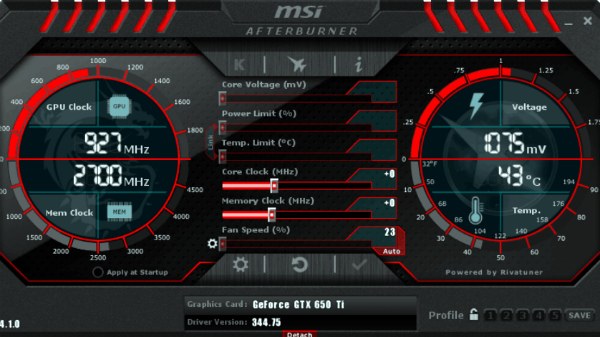
\includegraphics[width=0.6\textwidth]{msiafterburner.jpg}
\caption{MSI Afterburner}
\label{fig:msi}
\end{figure}

O \textit{Clock Speed} é o número de ciclos por segundo que acontecem nos \textit{cores}. Por exemplo, se uma \ac{gpu} tiver um \textit{Core Clock} de 1000MHz, isto quer dizer que os \textit{cores} oscilam 1,000,000 de vezes por segundo. 

Esta característica determina a eficácia de uma \ac{gpu} a realizar as suas tarefas. Geralmente, este é o fator que diferencia sistemas que operam com as mesmas \acp{gpu} ({\footnotesize no caso de haverem modificações no \textit{Core Clock} feitas pelo utilizador ou pelo fabricante}). É também utilizado para calcular o potencial de renderização de gráficos da Placa de Vídeo.
\clearpage

\subsection{VRAM}
\label{sec.mem}
Este componente é o segundo mais importante de uma placa de Vídeo. \ac{vram} é onde todos os dados gráficos e textura de jogos são armazenados para serem processados pela \ac{gpu}. É de notar que maior velocidade da \ac{vram} aumenta drasticamente a performance da \ac{pg}, mas apenas se a \ac{gpu} não for fraca e consiga acompanhar. Memória por si própria não aumenta o desempenho da \ac{pg}.

\begin{figure}[h]
\centering
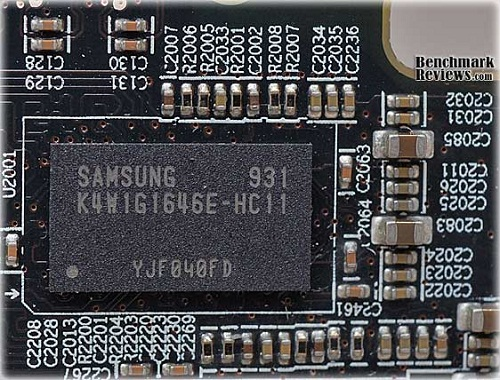
\includegraphics[width=0.5\textwidth]{mem.jpg}
\caption{VRAM}
\label{fig:vram}
\end{figure}

Há vários tipos de \ac{vram} disponíveis para Placas de Vídeo dependendo na velocidade e banda larga que oferecem:
\begin{enumerate}
  \item DDR3
  \item HBM
  \item HBM2
  \item GDDR5X
  \item GDDR5
  \item GDDR6
  \item GDDR6X
\end{enumerate}

A DDR3 é a mais antiga e consequentemente, a mais lenta, utilizada em \acp{pg} de baixa gama. A GDDR5 é a mais popular e utilizada em \acp{pg} de média gama. A GDDR6X é utilizada nas \acp{pg} de topo de gama da \textit{Nvidia}
\clearpage
 %%%%%%%%%%%%%%%%%%%%%%%%%%
\subsection{VRM}
\label{sec.vrm}
Talvez o terceiro componente mais importante da \ac{pg}, o Módulo regulador de voltagem ou ,\ac{vrm}, é o circuito que fornece energia à \ac{gpu}. O \ac{vrm} converte a voltagem de grande nível(12V) proveniente da Fonte de Alimentação ou \ac{psu}\footnote{Componente do Computador que fornece energia ao sistema} para níveis mais baixos de voltagem(1 a 1,5V), visto que a \ac{pg} opera nestes níveis de tensão.
\begin{figure}[h]
\centering
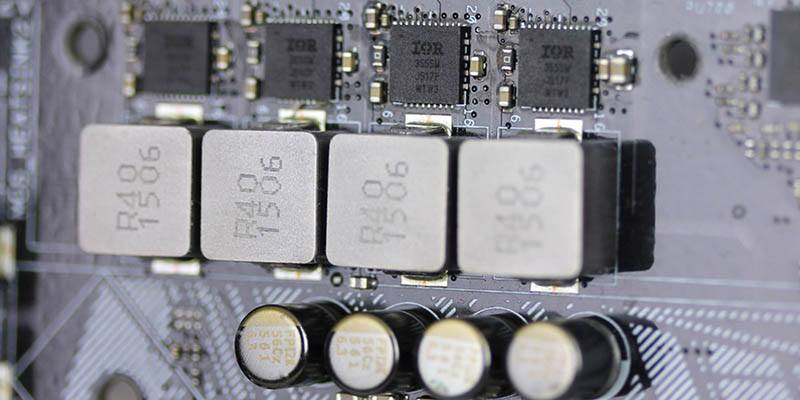
\includegraphics[width=0.5\textwidth]{vrm.jpg}
\caption{VRM}
\label{fig:vrm}
\end{figure}

O número de Reguladores de Voltagem numa placa de vídeo variam de produto para produto, dado que há \acp{pg} com diferentes graus de performance e com necessidades de energia diferentes. \acp{vrm} podem chegar a temperaturas ainda maiores que a \ac{gpu}, sendo necessários agentes de refrigeração para prevenir danos permanentes a \acp{pg}.


\clearpage
%%%%%%%%%%%%%%%%%%%%%%%%%%
\subsection{Cooler}
\label{sec.cooler}

Todas as placas de vídeo possuem um tipo de Cooler para dissipar o calor e manter as temperaturas da \ac{gpu}, \ac{vram} e \ac{vrm} em níveis seguros. Os Coolers podem ser considerados ativos ou passivos. Os Coolers ativos possuem um \textit{heatsink} e ventoinha(Figura) enquanto que os Coolers passivos possuem apenas o \textit{heatsink}. Existem também \textit{Water Coolers}, ou seja, Coolers que arrefecem o sistema através de água e geralmente são encontrados nas \acp{pg} do mais alto nível.


\begin{figure}[h]
     \centering
     \begin{subfigure}[b]{0.3\textwidth}
         \centering
         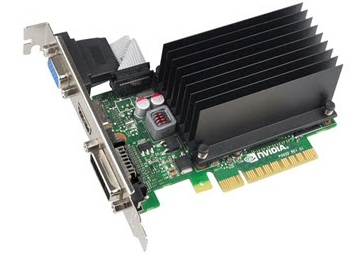
\includegraphics[width=\textwidth]{heatsink.png}
         \caption{Cooler com Heatsink}
         \label{heats}
     \end{subfigure}
     \hfill
     \begin{subfigure}[b]{0.3\textwidth}
         \centering
         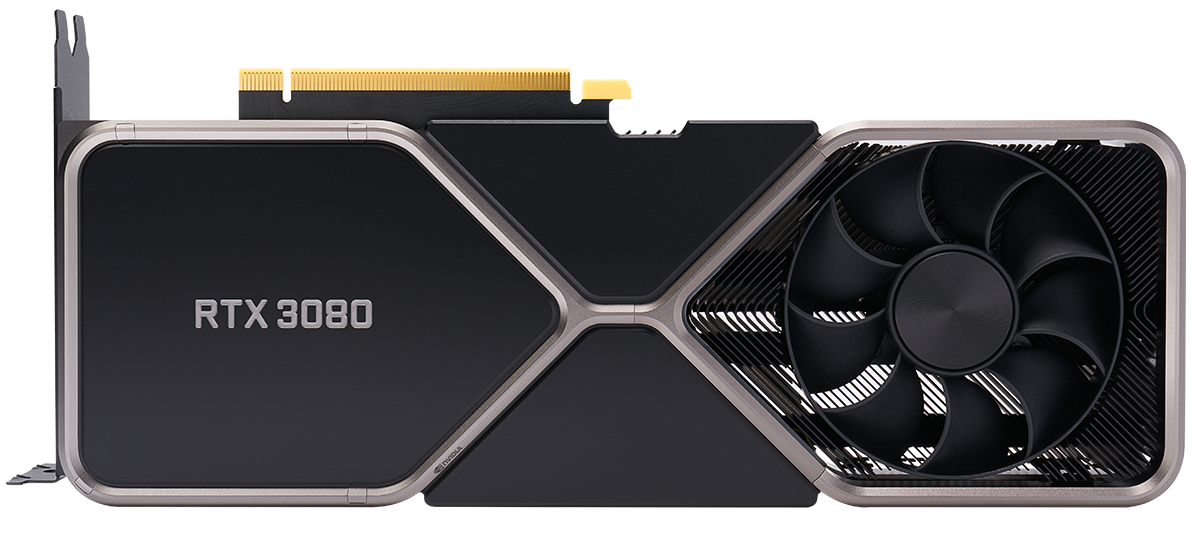
\includegraphics[width=\textwidth]{faneheatsink.png}
         \caption{Cooler com Heatsink e ventoinha}
         \label{heatvent}
     \end{subfigure}
     \hfill
     \begin{subfigure}[b]{0.3\textwidth}
         \centering
         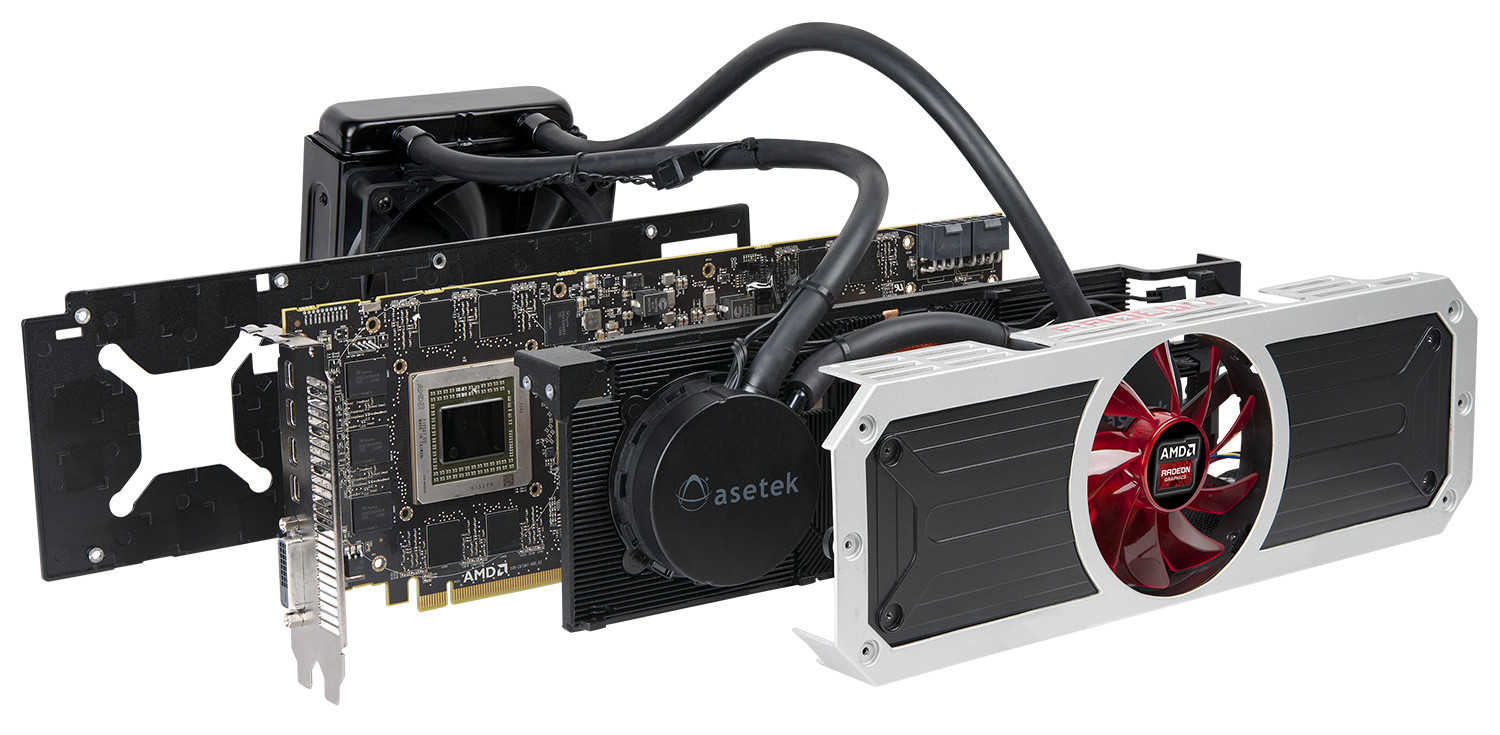
\includegraphics[width=\textwidth]{cooler.jpg}
         \caption{Water Cooler}
         \label{fig:five over x}
     \end{subfigure}
        \caption{Diferentes Tipos de Cooling}
        \label{watercooler}
\end{figure}

A maioria das \acp{pg} apresentam Coolers do tipo ativo, porque geralmente, requerem menos espaço e produzem melhor dissipação de calor, enquanto que Cooling passivo é utilizado em \acp{pg} de baixa qualidade e é completamente silencioso a realizar a sua função.
\clearpage

\subsection{PCB}
\label{sec.pcb}

O Circuito Impresso ou \ac{pcb} é a base onde componentes como \ac{gpu}, \ac{vram}, \ac{vrm}, Sensores, entre outros, estão montados. Placas de Vídeo de alta gama costumam possuir um \ac{pcb} mais comprido.

\subsection{Conectores}
\label{sec.conec}
\subsubsection{PCI Express x16}
O \ac{pcie} é o único local de comunicação entre a placas de vídeo e a placa-mãe\footnote{Parte do computador que serve como plataforma para conectar e interligar todos os componentes} e o \ac{cpu} e está presente em todas as \acp{pg} modernas.

\begin{figure}[h]
\centering
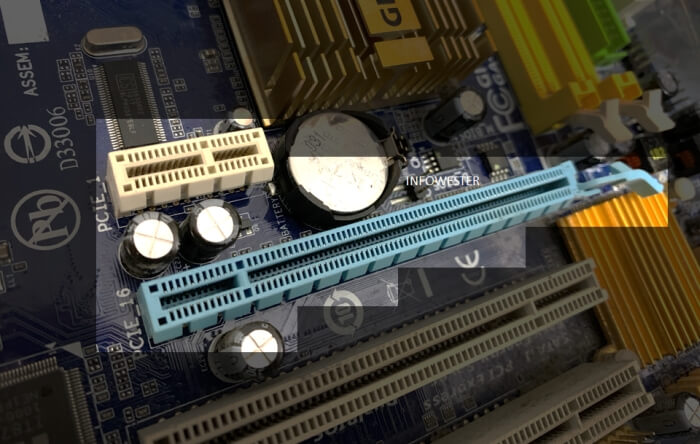
\includegraphics[width=0.5\textwidth]{pcie16.jpg}
\caption{PCI Express}
\label{fig:pcie}
\end{figure}

O \ac{pcie} x16 fornece até 75 Watts de potência à placa de vídeo.
\clearpage
\subsubsection{6-Pin e 8-Pin PCI-E}

As \acp{pg} que apresentam um maior nível de consumo de eletricidade necessitam de mais potência proveniente da \ac{psu} através de conectores 6-pin ou 8-pin(\autoref{fig:pin}).

\begin{figure}[h]
\centering
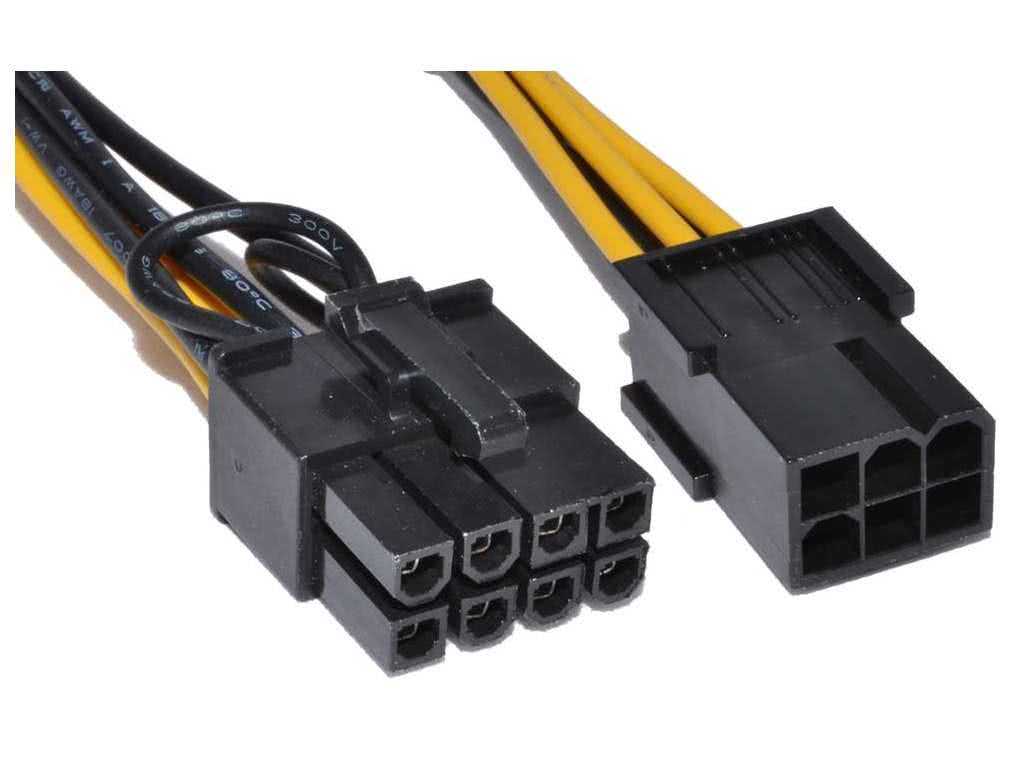
\includegraphics[width=0.5\textwidth]{6-8-pin.jpg}
\caption{Conectores 6-pin e 8-pin}
\label{fig:pin}
\end{figure}

Algumas placas de vídeo têm apenas conectores 6-pin, outras têm apenas 8-pin e algumas de topo de gama apresentam ambos os conectores.

Um conector 6-pin pode fornecer 75 Watts de potência à \ac{pg} e um conector 8-pin pode fornecer 150 Watts.
\clearpage
\subsubsection{Display Connector}
Todas as placas de vídeo têm \textit{display ports} para serem conectadas ao monitor utilizando o \textit{Display Connector}.

Existem vários tipos de \textit{display ports}:
\begin{enumerate}
  \item VGA
  \item DVI
  \item HDMI
  \item DP 
\end{enumerate}

VGA é a tecnologia mais antiga da lista, ou seja, suporta apenas resoluções mais pequenas enquanto que os conectores DVI, HDMI e DP suportam resoluções maiores e com mais clareza de imagem.

\begin{figure}[h]
\centering
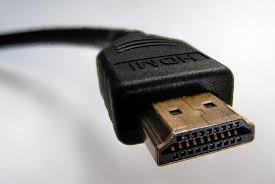
\includegraphics[width=0.5\textwidth]{hdmi.jpg}
\caption{Conector HDMI}
\label{fig:hdmi}
\end{figure}
\clearpage

\subsubsection{Conector de SLI/CrossFire}
Existem \acp{pg} que podem ser utilizadas ao mesmo tempo num computador, acabando por aumentar drasticamente a performance geral.

Estas \acp{pg} apresentam um SLI\footnote{SLI é tecnologia da Nvidia} ou CrossFire\footnote{CrossFire é tecnologia da AMD} Slot montado no \ac{pcb}
e em sistemas utilizando duas ou mais placas de vídeo, as mesmas estão conectadas através do Conector de SLI ou CrossFire.


\begin{figure}[h]
     \centering
     \begin{subfigure}[h]{0.3\textwidth}
         \centering
         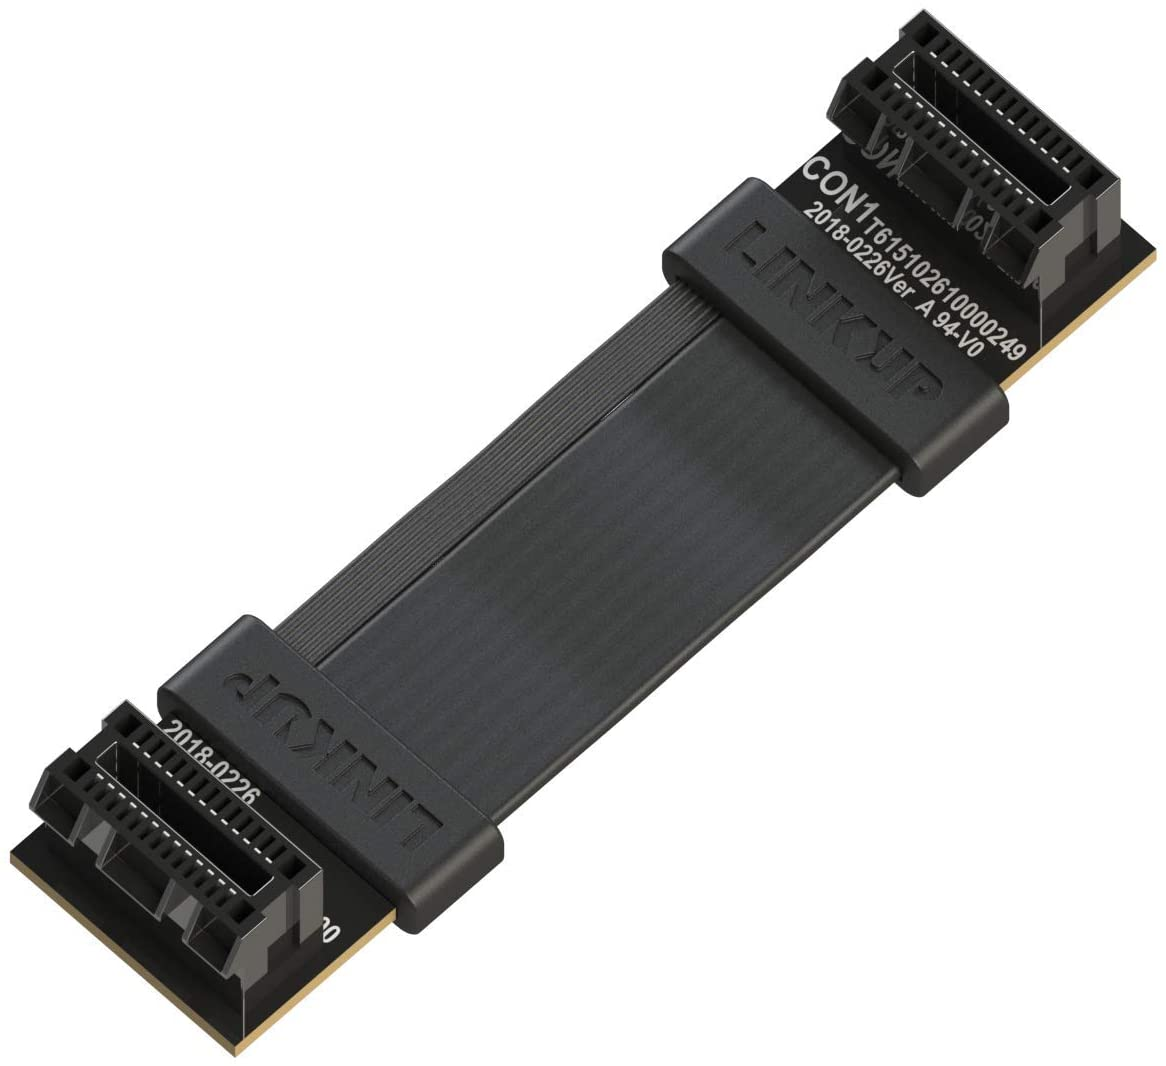
\includegraphics[width=\textwidth]{sli.jpg}
         \caption{Conector SLI}
         \label{fig:sli}
     \end{subfigure}
     \hfill
     \begin{subfigure}[h]{0.3\textwidth}
         \centering
         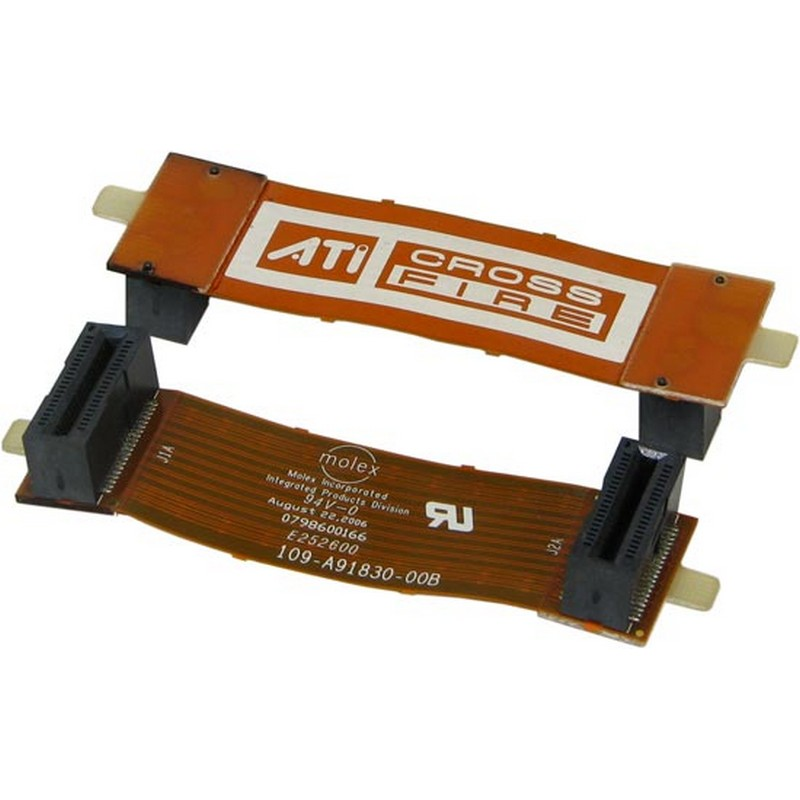
\includegraphics[width=\textwidth]{cf.jpg}
         \caption{Conector CrossFire}
         \label{fig:cf}
     \end{subfigure}
     \caption{Dois tipos de Conectores}
        \label{fig:slicf}
\end{figure}
\clearpage
\subsection{Controlador}

O Controlador, ou \textit{driver}, é essencialmente \textit{software} que trata da comunicação entre o sistema operativo, videojogos e aplicações e a Placa de Vídeo.

É extremamente importante que todas as Placas de Vídeo tenham este \textit{software} instalado e atualizado para assegurar que a \ac{pg} esteja a funcionar como é suposto e para evitar o encontro de erros.

\begin{figure}[h]
\centering
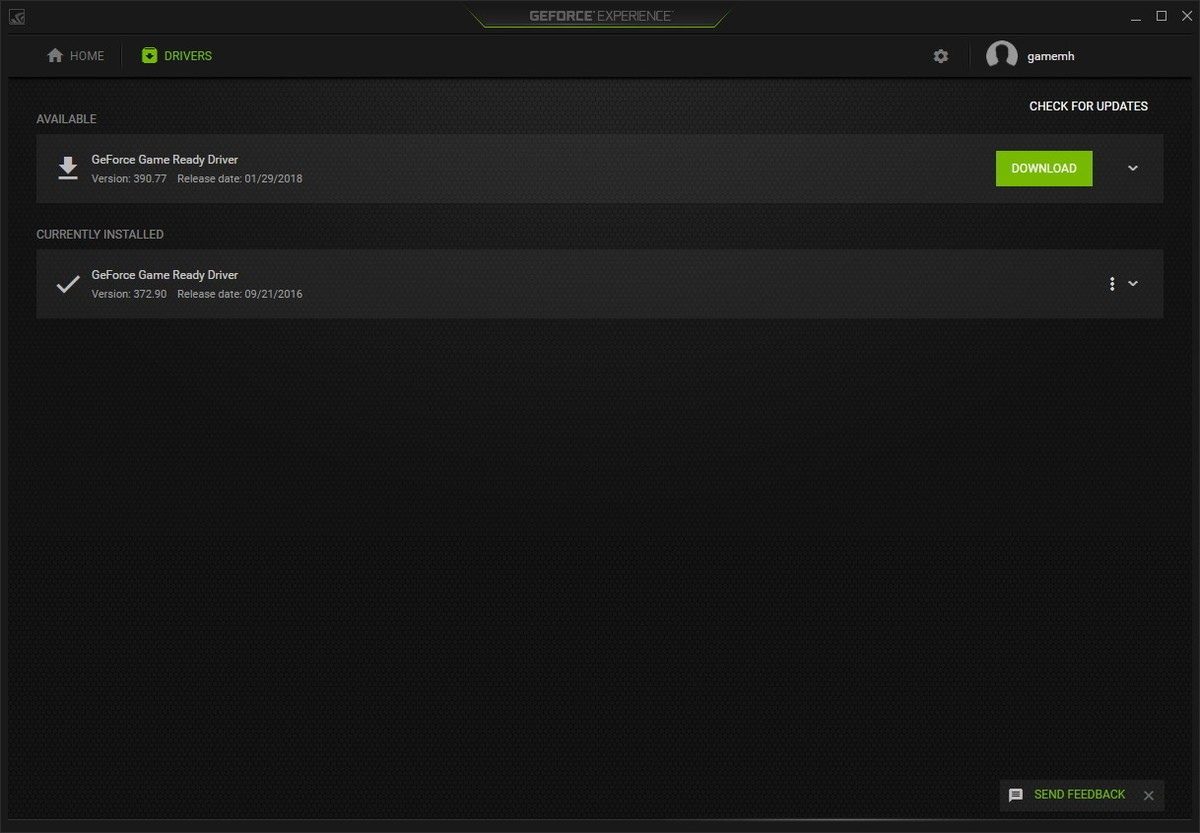
\includegraphics[width=0.5\textwidth]{nvidia.jpg}
\caption{Software de Controladores fornecido pela Nvidia}
\label{fig:nvidia}
\end{figure}

\begin{figure}[h]
\centering
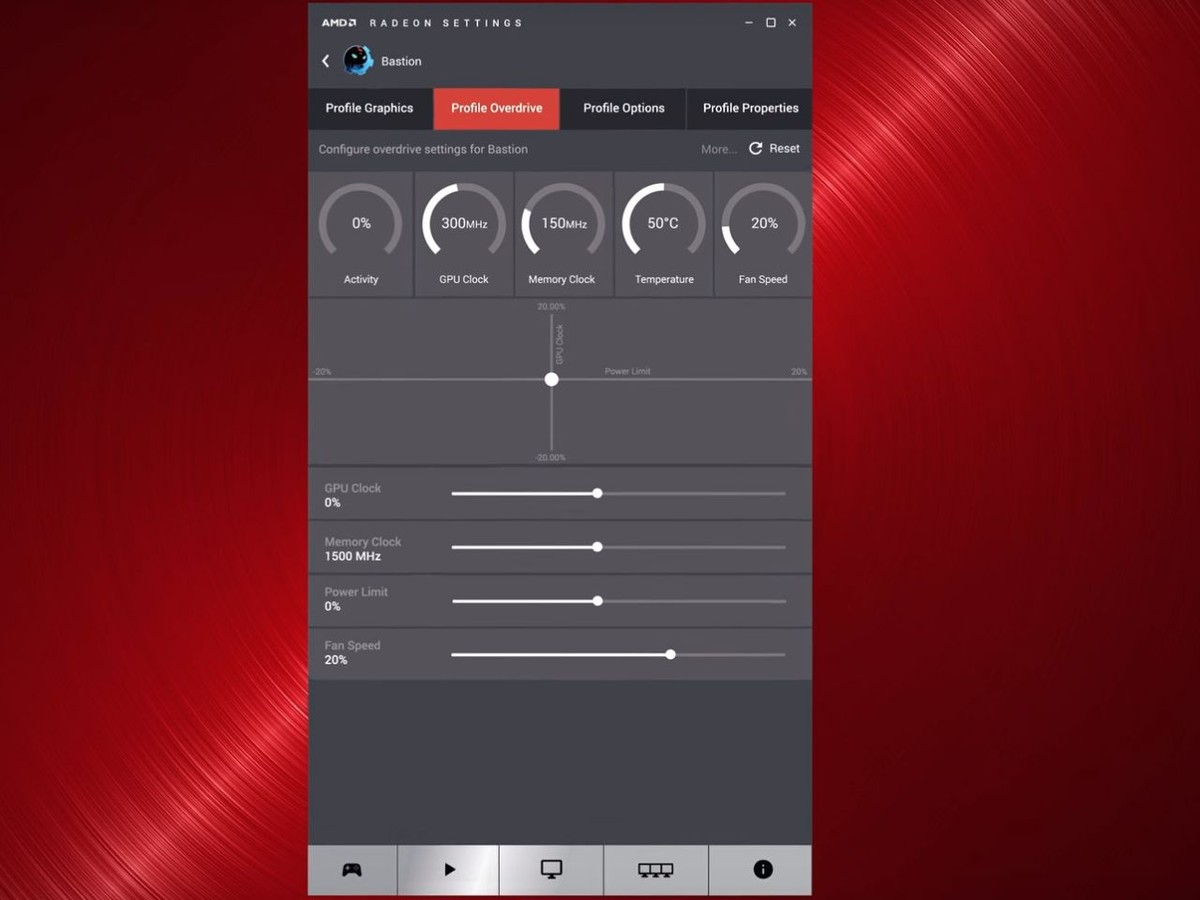
\includegraphics[width=0.5\textwidth]{amd.jpg}
\caption{Software de Controladores fornecido pela AMD}
\label{fig:amd}
\end{figure}


\chapter{Antes das Placas Gráficas}
\label{before}

Inicialmente, as \acp{pg} possuiam apenas um único \textit{core} em que se exercia uma funcão fixa utilizada apenas para gerar gráficos.
Como qualquer outro tipo de componente tecnológico, as placas gráficas têm-se tornado cada vez mais potentes e otimizadas de forma a acompanhar a evolução dos restantes componentes de um computador.

Nos dias de hoje, as \acp{pg} operam com um elevado conjunto de \textit{cores} realizando cálculos bastante complexos desde pesquisa de dados a inteligência artificial.

Atualmente, a \ac{pg} é um dos componentes mais importantes de \textit{hardware}, mas até 1999, com a criação da primeira Placa de Vídeo especializada, (a GeForce 256 da empresa Nvidia) não havia nenhum componente especializado de processamento de imagens semelhante aos que nós conhecemos atualmente. 
Sendo esta função tão essencial numa máquina, como era executado este cargo antes da \ac{pg}?

\clearpage
\section{1970s}

Na década de 1970, foram inventados os \textit{video shifters}\cite{shifter} e \textit{video address generators} com a função de transportar a informação proveniente do processador, ou \ac{cpu}, até à tela.
\begin{figure}[h]
\centering
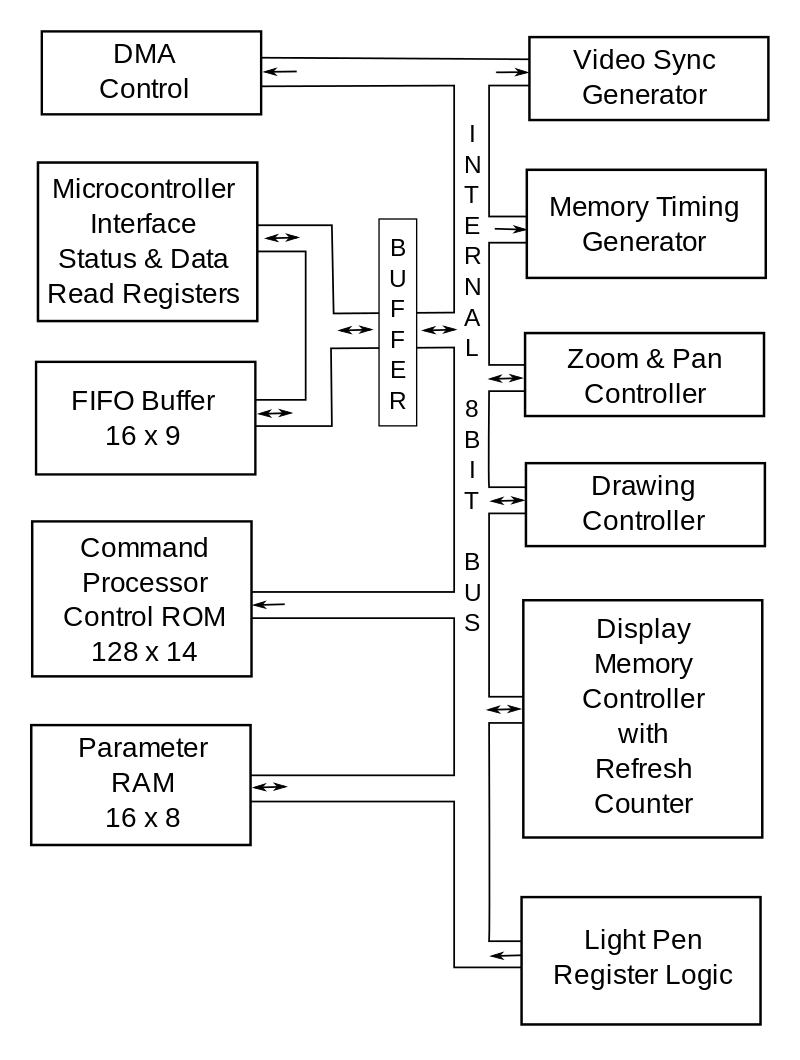
\includegraphics[width=0.35\textwidth]{videoadd.png}
\caption{Diagrama de blocos de um video shifter}
\label{fig:figure2}
\end{figure}

Portanto, antes desta tecnologia, as imagens eram processadas através do \ac{cpu} o que provava ser um processo bastante lento e ineficiente. 

Os \textit{video shifters}, utilizados maioritariamente em consolas de videojogos, apenas podem ser utilizados em jogos pré-selecionados estando programados para gerar somente as imagens pertencentes ao videojogo. Logo, não são considerados placas gráficas tradicionais.

Eram capazes de exibir imagem em 2D na resolução de 62 x 128 em preto e branco. (Para referência, o FULLHD, ou 1080p, tem a resolução de 1920 x 1080 e os monitores atuais são capazes de exibir milhões de cores.)
\clearpage

\vspace{10mm}

À medida que os sistemas operativos com \textit{interfaces} mais gráficas (\autoref{fig:os}) ganhavam popularidade, era exigida uma maior demanda por um melhor desempenho gráfico.

\begin{figure}[h]
\centering
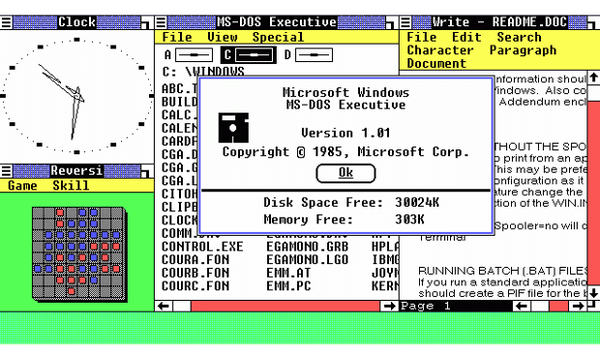
\includegraphics[width=0.5\textwidth]{windows.png}
\caption{Exemplo de Sistema Operativo da Época}
\label{fig:os}
\end{figure}

Em 1979, o sistema de \textit{arcade} Namco Galaxian (\autoref{fig:namco})foi lançado e possuia \textit{hardware} capaz de suportar cor RGB, \textit{tilemap backgrounds}, e vídeo costumizado. 

Foi um dos sistemas mais populares na sua era.

\begin{figure}[h]
\centering
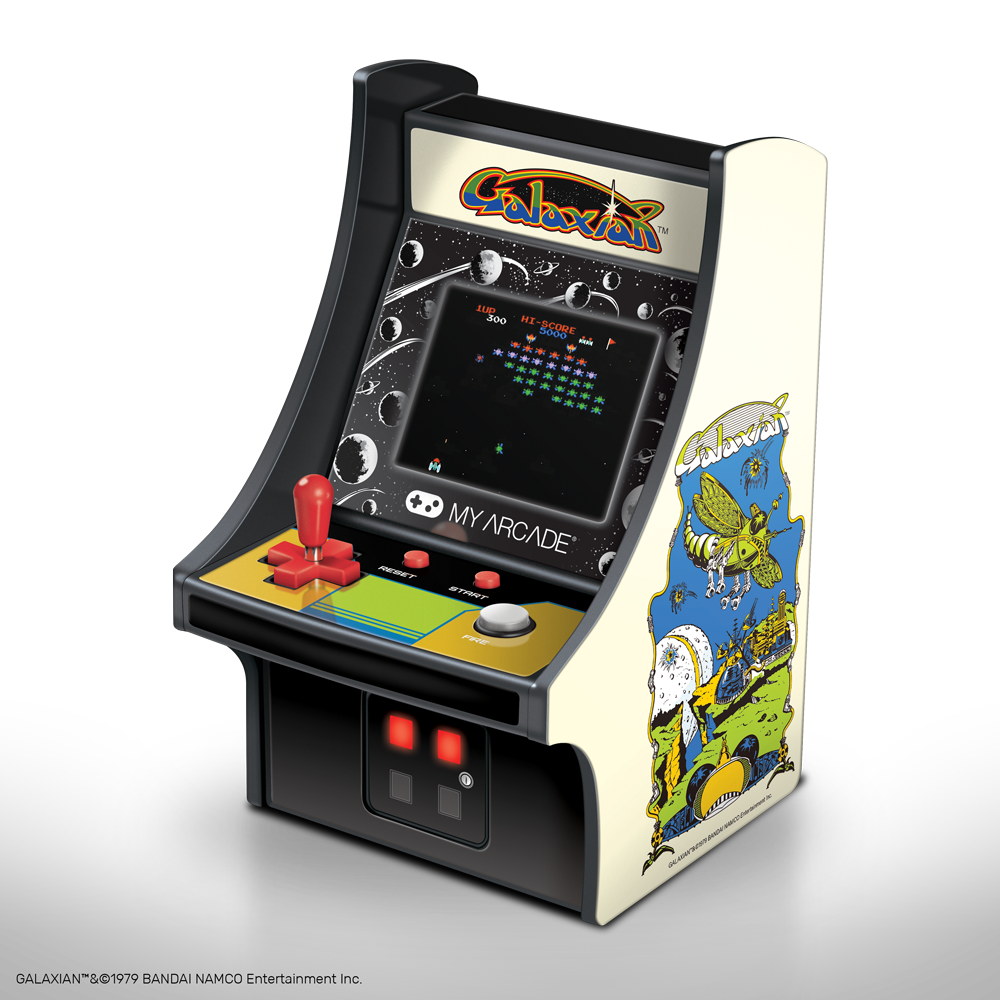
\includegraphics[width=0.5\textwidth]{namco.png}
\caption{Namco Galaxian}
\label{fig:namco}
\end{figure}
\clearpage
\section{1980s}

Na década de 1980, houve vários avanços na tecnologia de gráficos para videojogos como computadores. Foi inventado o primeiro processador de vídeo integrado para computadores, o NEC µPD7220 (\autoref{fig:nec}), que era capaz de desenhar linhas e círculos, e o primeiro processador de vídeo programável TMS34010. (\autoref{fig:tms})


\begin{figure}[h]
\begin{subfigure}{0.5\textwidth}
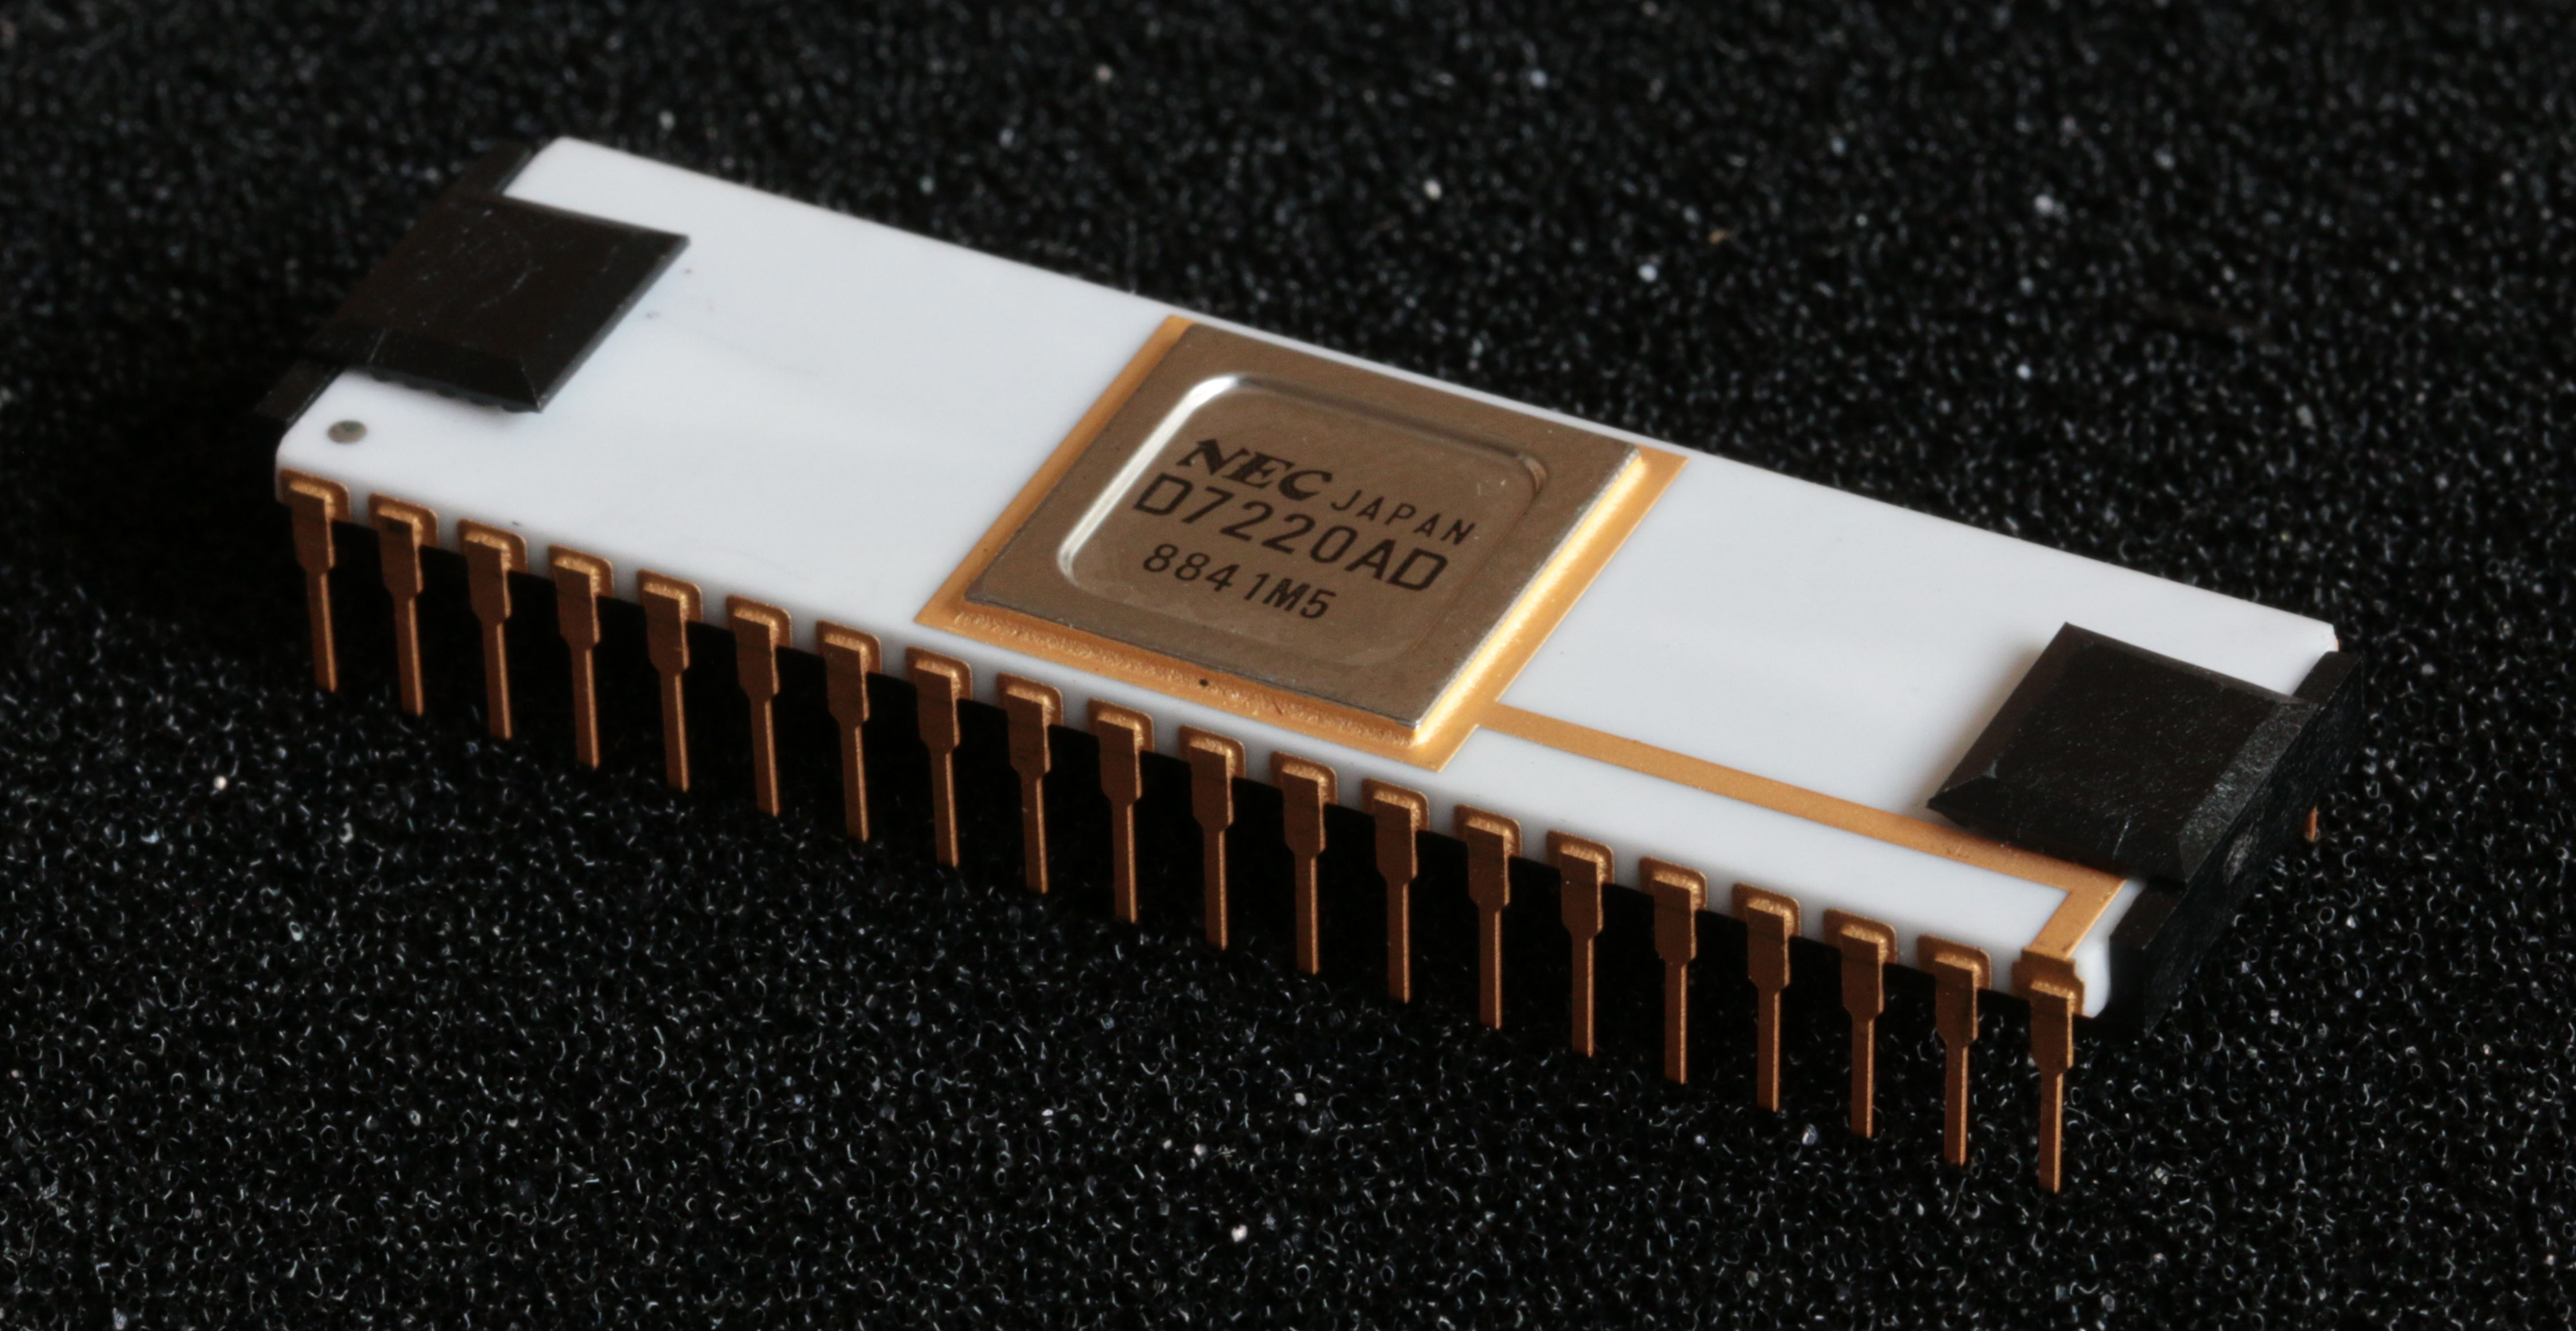
\includegraphics[width=0.9\linewidth, height=5cm]{nec.jpg} 
\caption{NEC µPD7220}
\label{fig:nec}
\end{subfigure}
\begin{subfigure}{0.5\textwidth}
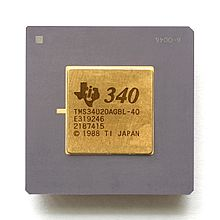
\includegraphics[width=0.9\linewidth, height=5cm]{tms.jpg}
\caption{TMS34010}
\label{fig:tms}
\end{subfigure}

\caption{Os primeiros avanços de 1980}
\label{fig:nectms}
\end{figure}

Mais do que nunca havia uma grande demanda por \textit{hardware} capaz de produzir gráficos, portanto cada vez mais empresas começaram a investir neste ramo.

Em 1981, a \ac{ibm}\footnote{Empresa norte-americana voltada para a informática} começou a incorporar adaptadores gráficos monocromáticos e de cores nos seus processadores de vídeo de forma a chegarem a uma melhor clareza de imagem e vídeo.
\clearpage
Pouco depois, a Intel\footnote{A Intel Corporation é uma empresa multinacional focada em tecnologia} lançou o \textit{ISBX 275 Video Graphics Controller Multimodule Board} (\autoref{fig:isbx}), capaz de apresentar 8 cores numa resolução de vídeo de 256x256 e monocromático a 512x512.

\begin{figure}[h]
\centering
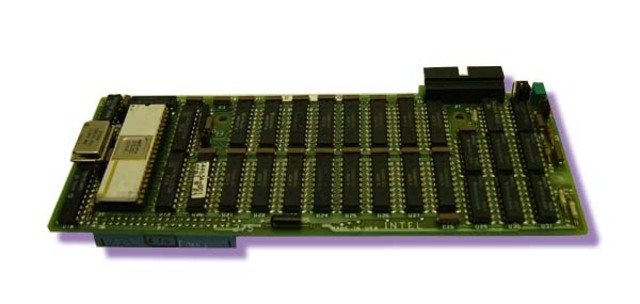
\includegraphics[width=0.5\textwidth]{isbx.jpg}
\caption{ISBX 275}
\label{fig:isbx}
\end{figure}

Entretanto, quatro emigrantes de Hong Kong, Lee Ka Lau, Francis Lau, Benny Lau, e Kwok Yuen Ho fundaram a ATI Technologies, que posteriormente criaram Placas de Vídeo revolucionárias que lideraram o mercado durante anos. 
\clearpage
\section{1990s}

Pela década de 1990, a demanda exigia gráficos 3D em tempo real, focando-se maioritariamente em videojogos. Quem liderava a inovação pela maioria da década foi a 3dfx\footnote{3dfx Interactive foi uma empresa norte-americana que produzia processadores de vídeo para 3D}, cujo primeiro produto, o Voodoo 1 (\autoref{fig:voodoo1}), suportava gráficos 3D e rapidamente alcançou 85\% do mercado\cite{market}. oodoo 1, como o Voodoo Graphics seria conhecido, se distingüia pela sua falta de um controlador de vídeo, necessitando uma placa VGA dedicada e um slot PCI a mais. A placa Voodoo só entrava em ação quando o PC em que estava instalada executava um aplicativo programado para usar a placa

\begin{figure}[h]
\centering
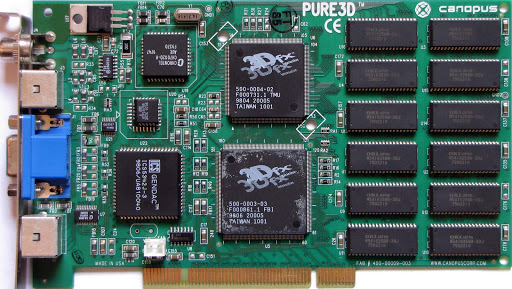
\includegraphics[width=0.5\textwidth]{voodoo1.jpg}
\caption{Voodoo 1}
\label{fig:voodoo1}
\end{figure}

A Voodoo 1 não era considerada uma Placa de Vídeo tradicional pelo facto de apenas conseguir gerar gráficos 3D. Então, para aplicações normais 2D, era necessário o uso de um controlador para \textit{software} 2D, uma placa VGA e um \textbf{slot} PCI a mais. Era também necessário o uso de uma aplicação instalada no computador para que a Voodoo 1 entrasse em ação.
\vspace{5mm}

Chegando ao fim do milénio, a Nvidia entrou no negócio das Placas de Vídeo lançando duas \acp{pg} revolucionárias, a Riva TNT 2, que suportava cor a 32 bits, e a GeForce 256, sendo esta considerada a primeira unidade de processador gráfico do mundo. 

Rapidamente se percebeu que estas \acp{pg} eram a próxima geração no que toca a processadores de vídeo. A performance obtida em videojogos e aplicações 3D, a qualidade de imagem e o preço eram suficientes para acabarem com a competição e logo se tornou no melhor produto nos olhos dos consumidores. Depois do seu lançamento, a qualidade gráfica dos videojogos aumentou exponencialmente.

\chapter{Mercado das Placas Gráficas}
\section{Rivalidade entre empresas}

Embora as placas gráficas nos acompanhem no nosso dia a dia há quase 40 anos, a sua especialização apenas começou no final do século XX. Novas marcas foram aparecendo e desaparecendo, mas as duas que fizeram questão de marcar a sua presença foram a Nvidia Corporation e a ATI Technonogies, futuramente comprada pela AMD. Começou então a longa disputa entre ambas as empresas, cuja competição já existe há cerca de duas décadas.

\vspace{5mm} Como referido no capítulo anterior, a primeira placa gráfica especializada, GeForce 256, foi criada pela NVidia, que para além de ter um grande reconhecimento por ter sido a pioneira do mercado das placas gráficas, também tem mantido uma enorme reputação quanto à qualidade dos seus produtos. Embora outras empresas tal como a Intel e AMD tenham criado também diversos modelos que mantinham a competição, a Nvidia ainda nos seus primeiros "anos de vida" acabara por se tornar numa empresa maioritariamente dedicada em criar placas gráficas, enquanto a Intel e AMD são mais reconhecidas pela grande qualidade dos seus processadores.

\vspace{5mm} Apesar da Intel ainda fabricar alguns produtos, costumam ser alternativas mais baratas e práticas. Por ser uma empresa tão popular na área dos processadores, optou por fabricar modelos de placas gráficas integradas nos próprios processadores, sendo por isso melhores escolhas para trabalhos mais básicos do dia à dia. Para além do preço, as placas gráficas integradas ocupam também menos espaço, por estarem inseridas num outro componente e também são ótimas opções quando o utilizador depende bastante da bateria, visto que conseguem adaptar o uso destas placas gráficas dependendo exclusivamente das funções que o utilizador realiza, onde trabalhos mais leves que necessitem de um menhor desempenho da placa gráfica gastem menos bateria, e vice-versa.

\vspace{5mm} Já a AMD, que embora considerada por muitos inferior à rival Nvidia, continuou a trazer grandes produtos para o mercado, e mesmo as últimas gerações de placas gráficas desenvolvidas pela AMD têm mudado algumas opiniões e mais do que nunca criado um clima de disputa entre as duas maiores marcas. Para além disso, consolas como PS4, Xbox One es a mais recentes PS5 e Xbox Series X apresentam placas gráficas AMD adaptadas. A realidade por detrás da maioria das opiniões negativas das placas Radeon criadas pela AMD deve-se não à inferioridade ou incompetência da empresa, mas principalmente de alguma ignorância dos próprios consumidores. É certo que durante alguns anos houveram diversas críticas às placas da AMD, quer pelo seu fraco período de vida, como os problemas trazidos quer por falta de atualização de drivers, quer por versões que apresentavam algum tipo de incompatibilidade. Apesar desses problemas terem sido resolvidos, os consumidores continuaram a ter uma fraca visão da empresa, baseando-se em eventos passados e considerando-os verídicos no presente. Felizmente para a empresa, a taxa de vendas tem vindo a aumentar e finalmente têm sido capazes de mostrar a qualidade do seu trabalho, criando assim ainda uma maior tensão entre Nvidia e AMD.

\section{Evolução Cronológica das Placas Gráficas}
Num mundo cheio de tecnologia, a inovação é a chave para garantir popularidade e, consequentemente, lucros para que uma empresa possa continuar a evoluir e voltar a inovar. A enorme popularidade tanto dos  vídeojogos como de programas de edição de imagem obrigaram a ser criadas novas formas de conseguir alcançar um elevado detalhe gráfico, que para tal, requerem componentes desenhadas especificamente para poderem satisfazer as necessidades desse público alvo. A performance em função do preço é dos aspetos, se não o aspeto mais tomado em conta na compra de uma placa gráfica. Algumas das placas gráficas mais populares até ao dia de hoje são:
\begin{itemize}
    \item \textbf{\#10:} Nvidia GeForce RTX 2070 SUPER
    \item \textbf{\#9:} AMD Radeon RX 580
    \item \textbf{\#8:} Nvidia GeForce GTX 1080
    \item \textbf{\#7:} Nvidia GeForce RTX 2060
    \item \textbf{\#6:} Nvida Geforce GTX 1660 Ti
    \item \textbf{\#5:} Nvida Geforce GTX 1650
    \item \textbf{\#4:} Nvida Geforce GTX 1070
    \item \textbf{\#3:} Nvida Geforce GTX 1050
    \item \textbf{\#2:} Nvida Geforce GTX 1050 Ti
    \item \textbf{\#1:} Nvida Geforce GTX 1060
\end{itemize}

\vspace{1cm}
\vspace{5mm} Um determinado modelo de uma placa gráfica pertence simultaneamente a uma determinada geração e série. Enquanto as gerações são apenas classificadas com o tipo de numeração ordinal, as séries são devidamente classificadas, e parte do nome dos modelos pertencentes a uma certa série dependem dela mesma. \newline
Enquanto as séries mais antigas possuiam quantidades de modelos mais restritas, hoje em dia elas uma única série pode possuir cerca de uma dezena de modelos. Geralmente os diferentes modelos de uma série de placas pode ser dividida em quatro grupos, consoante a unidade de processamento gráfico presente no modelo.

\vspace{5mm} Estes grupos são denominados \textbf{Entry-level}, para caracterizar as placas gráficas com GPU mais fraco da série, \textbf{Mid-range}, para as placas gráficas com uma performance intermédia, tendo um bom balanceamento entre atividades que requerem um maior desemepnho gráfico e outras operações mais simples, \textbf{High-end}, referente a placas gráficas de alto desempenho, desenhadas para situações profissionais ou elevada performance gaming e, por último, as \textbf{Enthusiast}, que possuem a melhor tecnologia que a empresa colocou nessa série. Obviamente que à medida que a qualidade do modelo aumenta, a quantidade de potência que uma fonte de alimentação deve possuir varia proporcionalmente.
\vspace{5mm}
\begin{figure}[h]
\centering
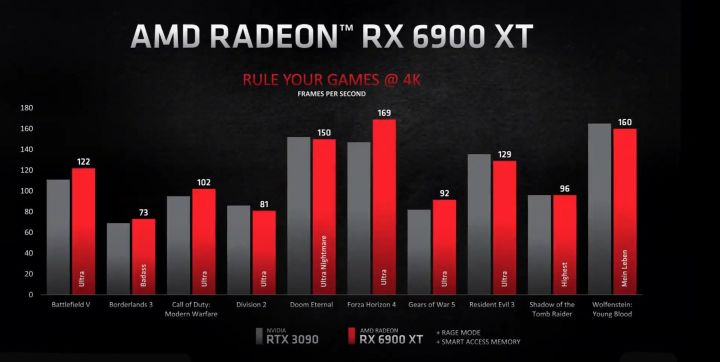
\includegraphics[width=0.5\textwidth]{comp.png}
\caption{Comparação entre a atual melhor placa gráfica de cada empresa}
\label{fig:comp}
\end{figure}

\begin{figure}[h]
\begin{subfigure}[b]{0.6\textwidth}
\centering
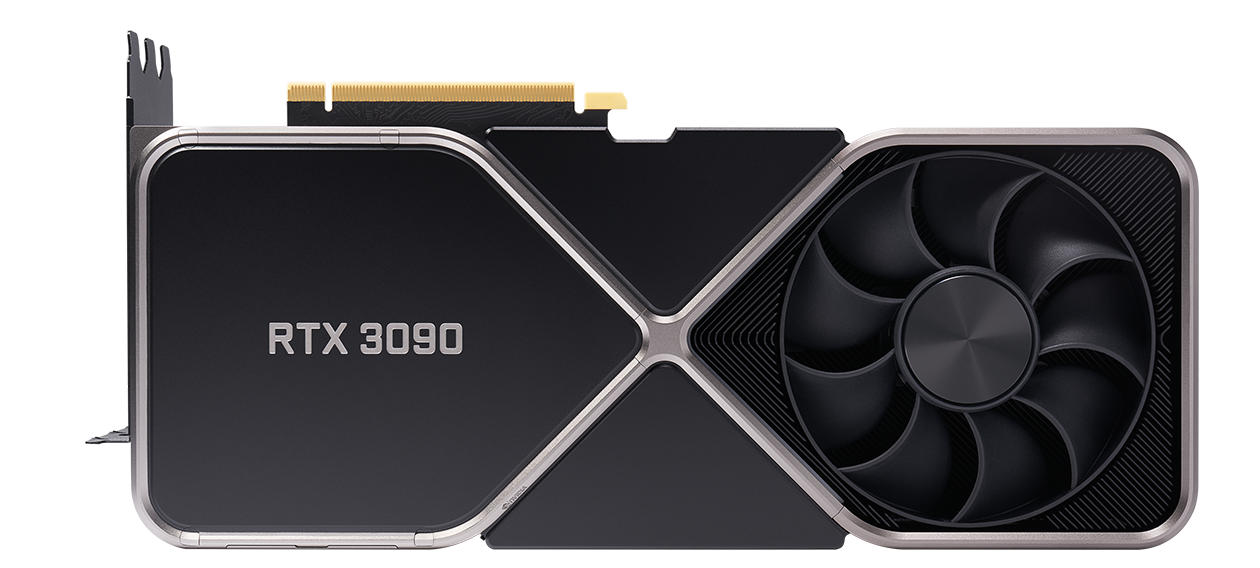
\includegraphics[width=0.5\textwidth]{rtx_3090.png}
\caption{Nvidia RTX 3090}
\label{fig:rtx3090}
\end{subfigure}
%
\begin{subfigure}[b]{0.6\textwidth}
\centering
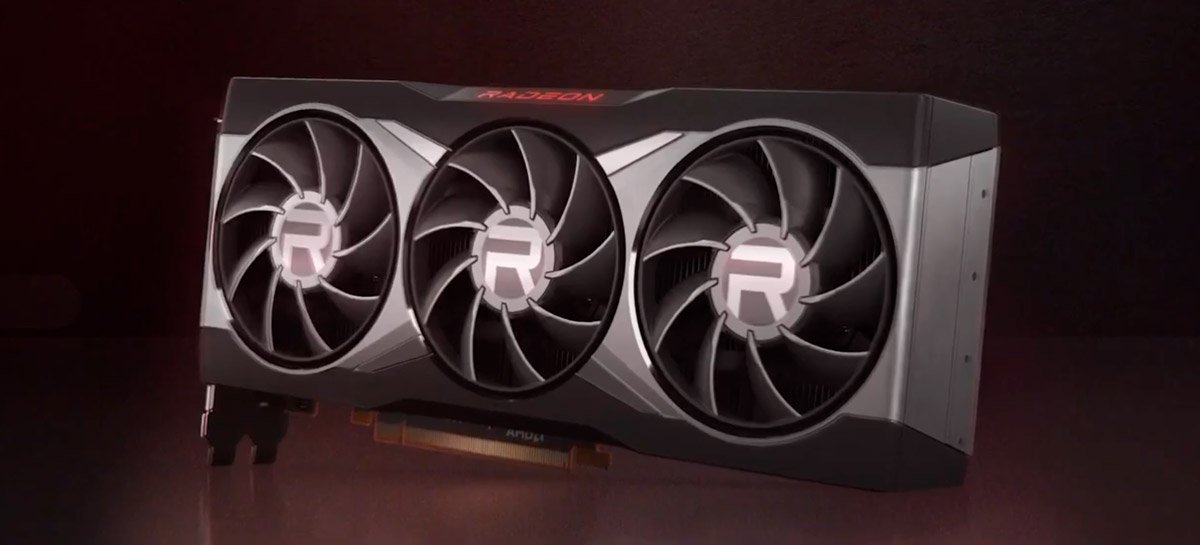
\includegraphics[width=0.5\textwidth]{radeon_rx_6900_xt.png}
\caption{Radeon RX6900 XT}
\label{fig:rx6900xt}
\end{subfigure}
\end{figure}

\vspace{3cm} A \autoref{tab:tab2} representa a evolução das séries de placas gráficas das maiores fabricadoras desde o seu primeiro lançamento até o presente ano. Os itens apresentados a \textcolor{orange}{laranja} representam variantes de outros modelos lançados anteriormente.

\vspace{8mm}
\begin{table}[h]
\centering
\begin{tabular}{|c|c|c|c|}\hline
    \multirow{2}{*}{\textbf{Ano}} & \multicolumn{3}{|c|}{\textbf{Fabricadora}} \\ \cline{2-4}
    & \textbf{Nvidia} & \textbf{ATI} & \textbf{AMD} \\ \hline
    \textbf{1999} & GeForce 256    & -              & -                      \\ \hline
    \textbf{2000} & GeForce 2      & Radeon R100    & -                      \\ \hline
    \textbf{2001} & GeForce 3      & Radeon R200    & -                      \\ \hline
    \textbf{2002} & GeForce 4      & Radeon R300    & -                      \\ \hline
    \textbf{2003} & GeForce FX     & -              & -                      \\ \hline
    \textbf{2004} & GeForce 6      & Radeon R400    & -                      \\ \hline
    \textbf{2005} & GeForce 7      & Radeon X1000   & -                      \\ \hline
    \textbf{2006} & GeForce 8      & -              & -                      \\ \hline
    \textbf{2007} & -              & Radeon HD2000  & -                      \\ \hline
    \multirow{2}{*}{\textbf{2008}} & GeForce 9      & \multicolumn{2}{|c|}{\multirow{2}{*}{Radeon HD5000}}     \\ \cline{2-2}
                                   & GeForce 200    & \multicolumn{2}{|c|}{} \\ \hline
    \multirow{2}{*}{\textbf{2009}} & \textcolor{brown}{GeForce 100}      & \multicolumn{2}{|c|}{\multirow{2}{*}{Radeon HD5000}}     \\ \cline{2-2}
                                   & \textcolor{brown}{GeForce 300}    & \multicolumn{2}{|c|}{} \\ \hline
    \multirow{2}{*}{\textbf{2010}} & GeForce 400    & \multirow{2}{*}{-}  & \multirow{2}{*}{Radeon HD6000}       \\ \cline{2-2}
                                   & GeForce 500    & \multirow{2}{*}{}   & \multirow{2}{*}{} \\ \hline
    \textbf{2011} & -              & -              & -                      \\ \hline
    \textbf{2012} & GeForce 600    & -              & Radeon HD7000          \\ \hline
    \multirow{2}{*}{\textbf{2013}} & \multirow{2}{*}{GeForce 700}    & \multirow{2}{*}{-}              & \textcolor{brown}{Radeon HD 8000} \\ \cline{4-4}
     & \multirow{2}{*}{} & \multirow{2}{*}{} & Radeon R\textit{x} 200 \\ \hline
    \multirow{2}{*}{\textbf{2014}} & \textcolor{brown}{GeForce 800M}    & \multirow{2}{*}{-}  & \multirow{2}{*}{-}       \\ \cline{2-2}
                                   & GeForce 900    & \multirow{2}{*}{}   & \multirow{2}{*}{} \\ \hline
    \textbf{2015} & -              & -              & Radeon R\textit{x} 300 \\ \hline
    \textbf{2016} & GeForce 10     & -              & Radeon RX 400          \\ \hline
    \multirow{2}{*}{\textbf{2017}} & \multirow{2}{*}{-}    & \multirow{2}{*}{-}              & \textcolor{brown}{Radeon RX 500} \\ \cline{4-4}
     & \multirow{2}{*}{} & \multirow{2}{*}{} & Radeon RX Vega \\ \hline
    \textbf{2018} & GeForce 20     & -              & -                      \\ \hline
    \multirow{2}{*}{\textbf{2019}} & \multirow{2}{*}{\textcolor{brown}{GeForce 16}}    & \multirow{2}{*}{-}              & Radeon RX 5000 \\ \cline{4-4}
     & \multirow{2}{*}{} & \multirow{2}{*}{} & \textcolor{brown}{Radeon 600} \\ \hline
    \textbf{2020} & GeForce 30     & -              & Radeon RX 6000         \\ \hline
    
\end{tabular}
\caption{Evolução das séries de placas gráficas\label{tab:tab2}}
\end{table}

%%%%%%%%%%%%%%%%%%%%%%%%%%%%%%%%%

\chapter{Para além das placas gráficas}
\section{Comunicação entre uma placa gráfica e um programa}
\subsection{Interface de programação de aplicações (\acs{api})}
A informação que é processada pela GPU, antes de conseguir alcançar um dispositivo de saída para que possa ser mostrada ao utilizador, tem que interagir com todos os softwares necessários de forma a transformar o código que saiu de placa gráfica para o código utilizado por um determinado programa. Sendo que cada componente de hardware tem uma linguagem base, programadores teriam que utilizar um tipo de linguagem diferente para cada configuração de hardware. Viu-se então a necessidade de criar uma forma de conseguir fazer com que hardware fosse capaz de interagir com software, processando a informação e a transmitindo-a para o utilizador. Foram então criadas interfaces que serviriam como intermediários entre o humano e a máquina, as \acs{api}. \cite{api}

\vspace{5mm}De uma forma mais simplificada, a driver da placa gráfica que o utilizador tiver no momento instalada vai ser a responsável por transmitir o código criado pela placa, essa informação vai ser então levada até um destinatário por uma \acs{api} utilizada pelo software que o utilizador quer interagir, tranformando a linguagem inicial numa outra linguagem. Obviamente não será um processo único, no caso de um utilizador que possua uma placa gráfica da Nvidia e que esteja a utilizador Windows 10, tenha o Google Chrome aberto numa rede social como o Instagram. De maneira simples, o código sairá da placa gráfica pela \acs{api} desenvolvida pela própria Nvidia, a CUDA, que foi desenhada para utilizar linguagens como C e C++, será levada para o sistema operativo, cuja \acs{api} é Win32 se o tipo de sistema operativo for de 32 bits ou Win64 caso seja de 64 bits, que está escrita em C, que por sua vez vai enviar a informação ao navegador de internet que pode estar escrito em C, C++, Javascript, Java ou Python e, por último, transmitindo o conteúdo para o website que utiliza apenas Python. \newline
Todos estes diferentes pontos por onde a informação navega podem ou não apresentar uma linguagem de programação diferente, e cabe aos \acs{api}s de conseguir adaptar de uma linguagem para outra, como exemplificado na \autoref{fig:api}. \newline

\begin{figure}[h]
\centering
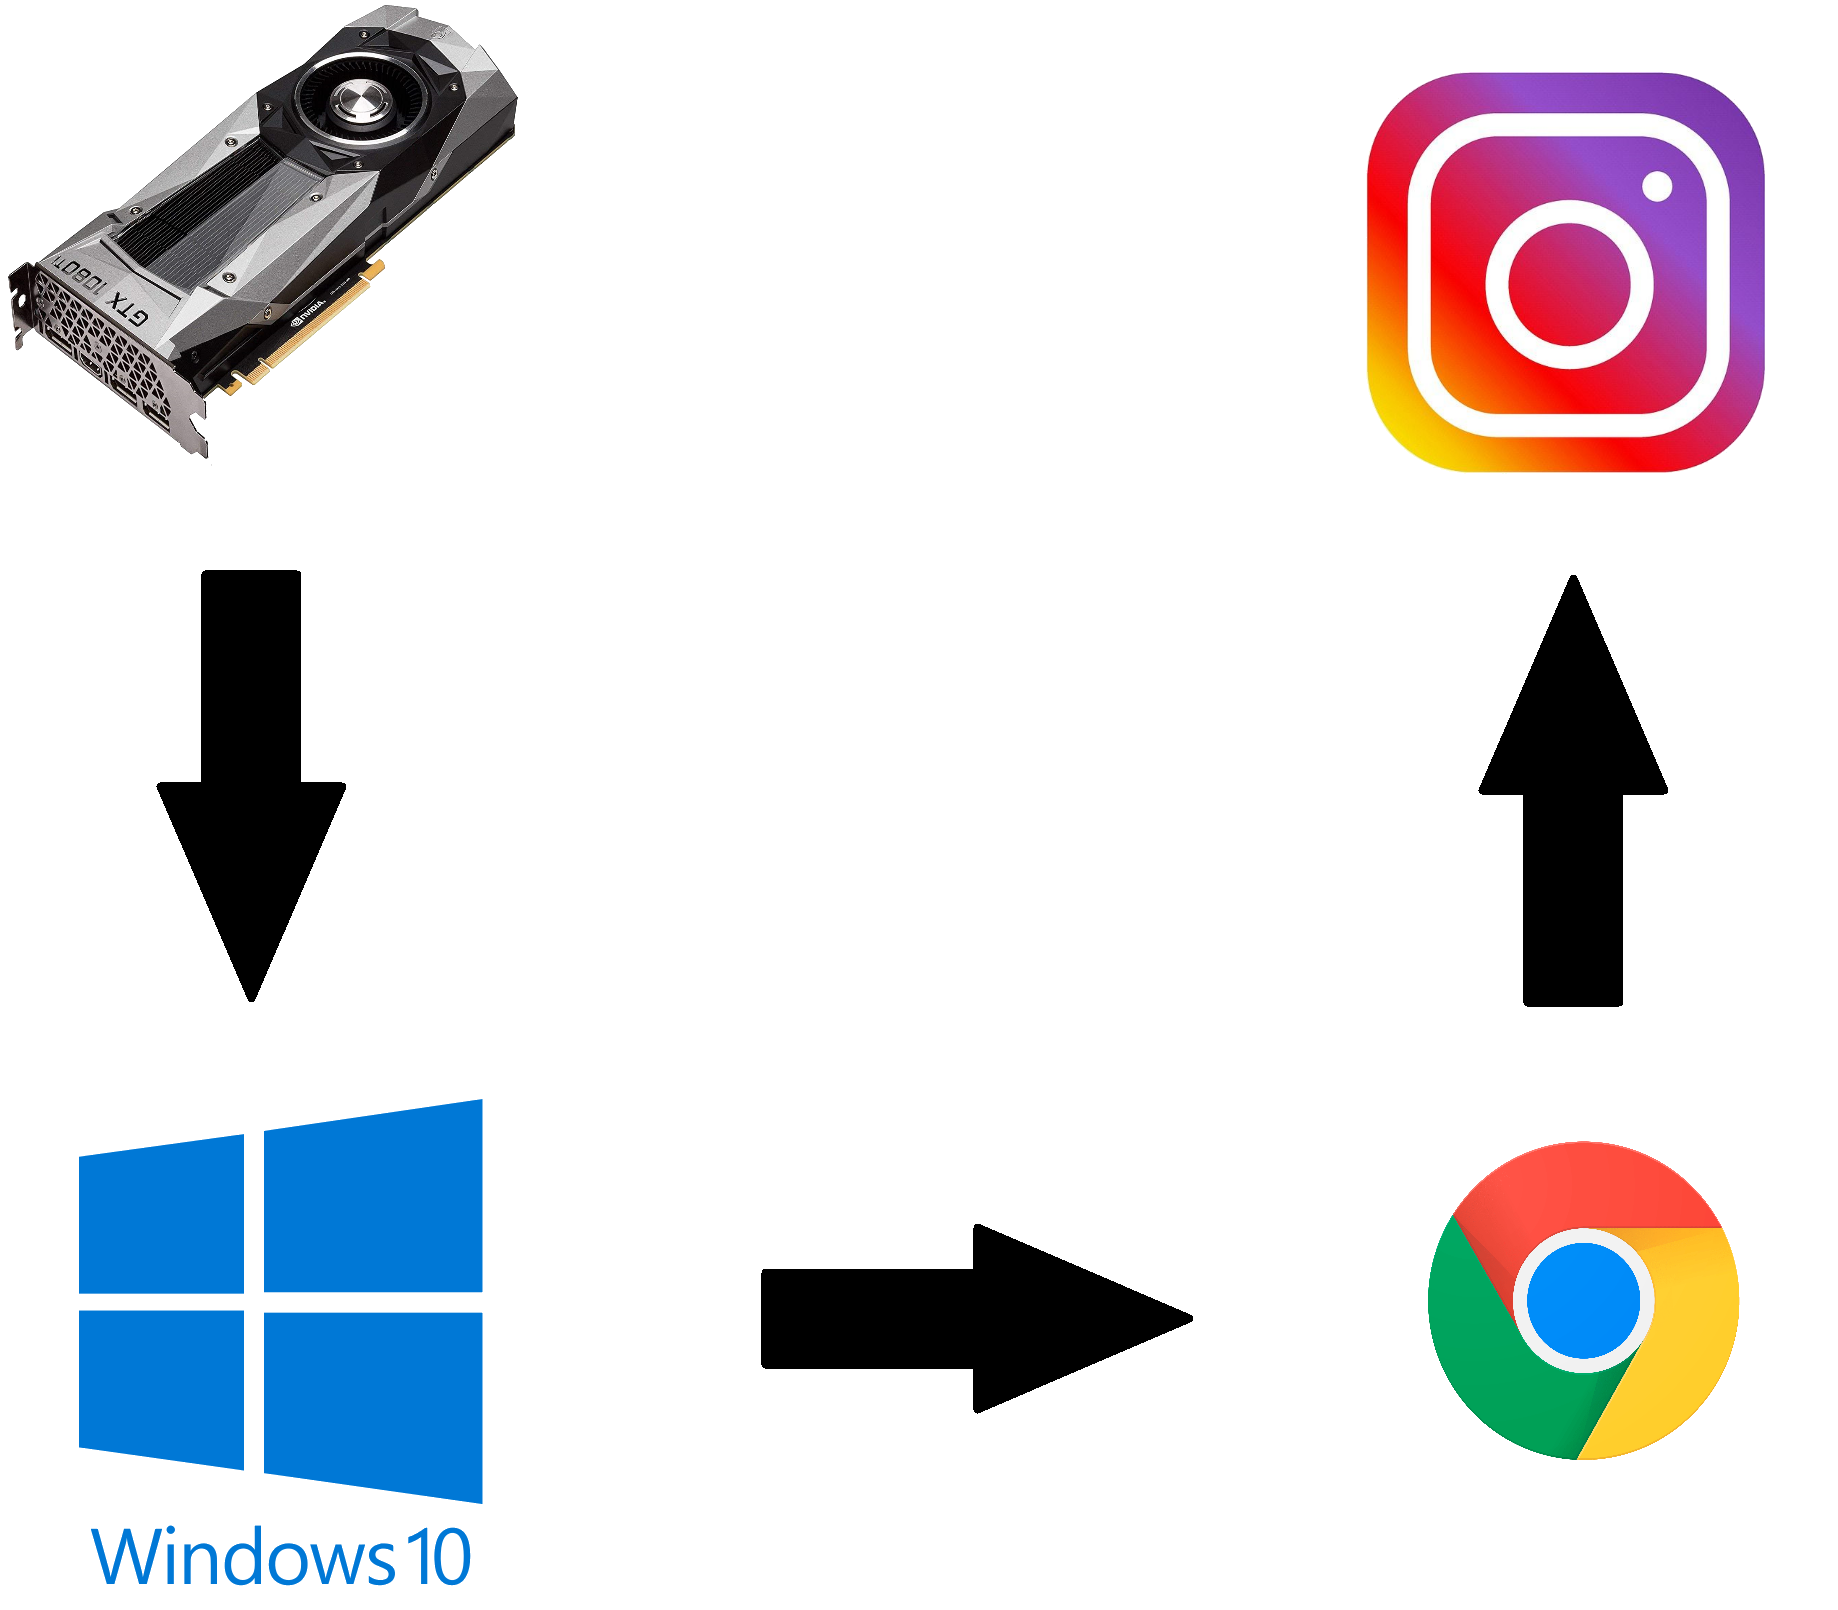
\includegraphics[width=0.5\textwidth]{api.png}
\caption{Exemplificação básica de como navega a informação desde o remetente até ao destinatário}
\label{fig:api}
\end{figure}

\subsection{APIs Gráficos} Como é de esperar, existem vários \acs{api}s especializados em determinadas áreas. Retratando a parte gráfica, alguns \acs{api}s que se destacam são a Vulkan, OpenGL, ambas desenvolvidas pela Khronos Group e a DirectX, desenvolvida pela Microsoft. Este último, possivelmente o mais conhecido dos três, é na verdade um conjunto de \acs{api}s integrados num só. \newline
Começando com OpenGL e DirectX visto serem as mais antigas, cada uma apresenta as suas vantagens e desvantagens, dependendo da finalidade do utilizador. A principal diferença é que a DirectX é exclusiva para Windows, pelo que qualquer outro sistema operativo ter-se-á a necessidade de utilizar OpenGL. Embora DirectX tenha a capacidade de trabalhar como um \acs{api} gráfico, com a componente Direct3D, ela suporta também áudio, DirectSound, controla todos os dispositivos de entrada, DirectInput, e implementação de técnicas de renderização, DirectX RayTracing (\acs{dxr}). \newline
Por ser especializada num só sistema operativo, a DirectX acabou por se tornar mais eficiente que OpenGL em Windows, sendo também a \acs{api} mais popular até ao presente dia. Para tal, a Khronos lançou uma nova \acs{api} como uma OpenGL mais contemporânea, a Vulkan.

\vspace{2cm} A nova \acs{api} trouxe otimizações que não eram possíveis serem alcançadas tanto pela OpenGL como pela DirectX, contudo, ainda é pouco utilizada, quer por ser mais complexa que DirectX quer por ser bastante nova e ainda apresentar alguns problemas. É no entanto uma enorme candidata ao futuro das APIs gráficas pela inovação na sua tecnologia, podendo um dia superar a própria DirectX tanto em performance como em popularidade.

\section{Raytracing e a renderização de imagens tridimensionais}
O Raytracing já é uma técnica antiga que começou a ser utilizada inicialmente na indústria cinematográfica, no entanto, é bastante recente na indústria dos videojogos. Ela tenta replicar a física realística do dia à dia com efeitos de iluminação, sombras e reflexos, variando apenas na forma como é transmitida quando comparada ao mundo real. Em vez de existir uma fonte de luz que vai incidir sobre um objeto e nos possibilita a sua visualização, a tecnologia RayTracing faz com dependendo do campo de visão do jogador, a luz viajará de forma inversa para o objeto, e do objeto procura a fonte emissora, criando assim as sombras e reflexos, que também irão depender de outros objetos e/ou fontes de iluminação. \newline \cite{nvidia}
Para além disso, a iluminação utilizando RayTracing é muito mais prática comparada aos métodos utilizados previamente de colocar toda a iluminação manualmente, representado na \autoref{fig:detroit_lum}, pelo facto de poder ser aplicada com código simples como na \autoref{fig:codigo_rt} que percorre todos os píxeis do ecrã, dando um determinado valor de iluminação a cada um deles e transmitindo uma claridade mais nítida e realista. \newline
\begin{figure}[h]
\centering
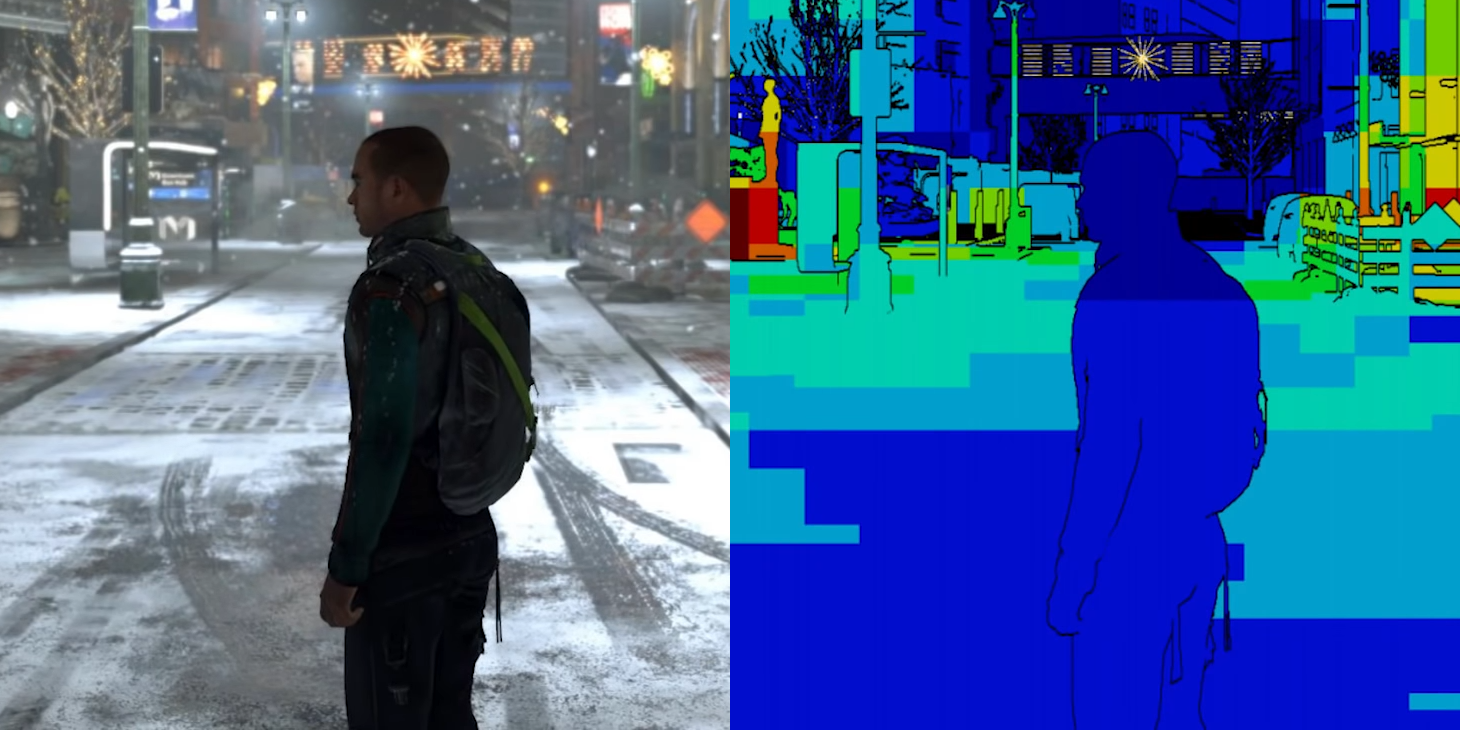
\includegraphics[width=1\textwidth]{detroit_lum.png}
\caption{O resultado final de um sistema de iluminação manual}
\label{fig:detroit_lum}
\end{figure}

\begin{figure}[h]
\centering
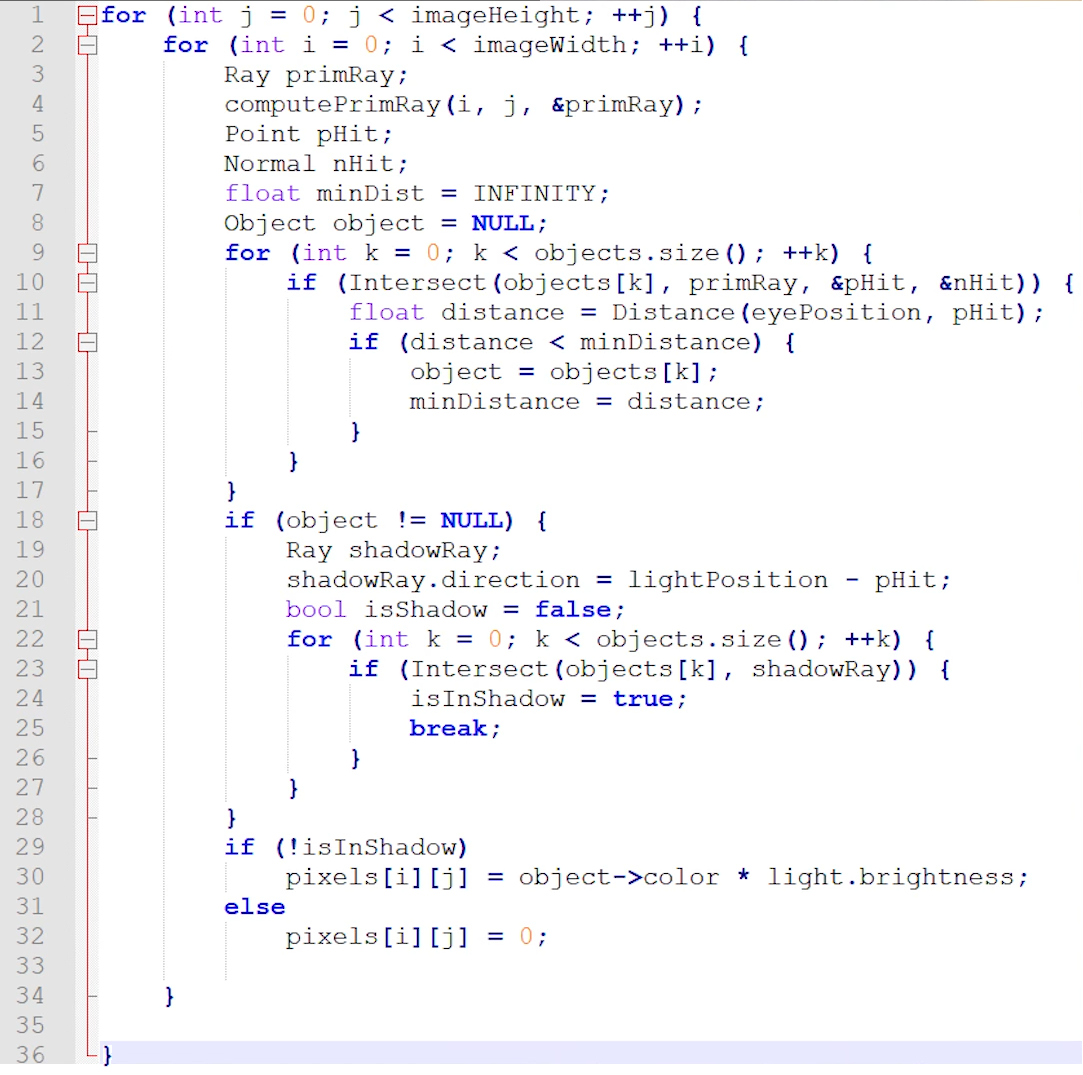
\includegraphics[width=1.4\textwidth]{codigo_raytracing.png}
\caption{Código simplificado na criação de RayTracing. Com cerca de 40 linhas de código, é finalmente possível criar o que já tinha sido imaginado há anos}
\label{fig:codigo_rt}
\end{figure}
\clearpage

\vspace{5mm} Por enquanto apenas as placas gráficas da Nvidia RTX (Séries GeForce 20 e 30) têm a capacidade de criar esses efeitos por natureza da própria placa, mas como referido anteriormente, a DirectX implementou na sua mais recente versão, DirectX 12, a extensão DirectX RayTracing, que integra completamente essa tecnologia na própria \acs{api}. Para além disso, é também completamente funcional em algumas placas gráficas para além das de modelo RTX, como as da geração anterior (Série GeForce 10), nas variantes das próprias RTX (Série GeForce 16) e ainda em placas gráficas AMD, cujos modelos que suportarão \ac{dxr} ainda se encontram por anunciar. \cite{directx}

\vspace{5mm} Embora o que se imaginava há bastante tempo finalmente se tenha tornado numa realidade, a tecnologia ainda apresenta bastantes limitações, pois não só é necessária a criação de uma placa gráfica capaz de a suportar, as próprias engines dos videojogos têm que as conseguir processar de forma a que não apresente nenhum defeito gráfico e sim que os melhore.

\begin{figure}[h]
\centering
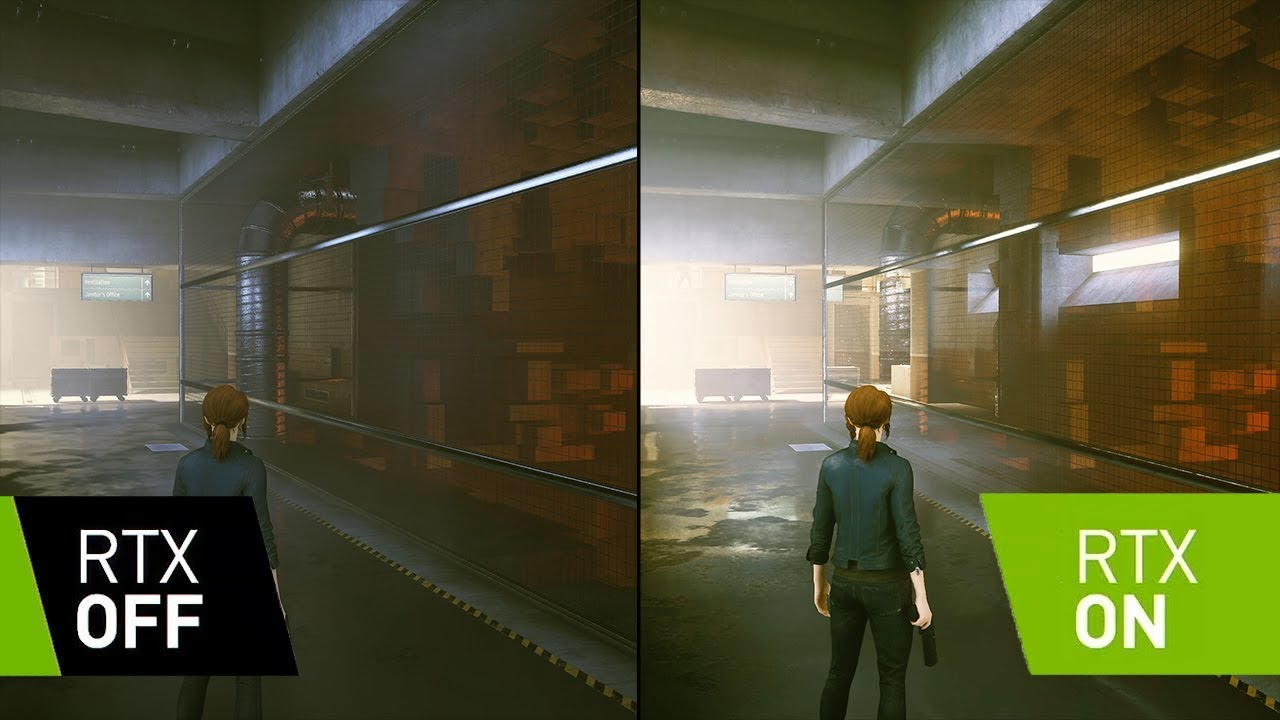
\includegraphics[width=1.2\textwidth]{rt_comp.jpg}
\caption{Influência do Ray Tracing nos videojogos}
\label{fig:rt_comp}
\end{figure}
\clearpage

%%%%%%%%%%%%%%%%%%%%%%%%%%%%%%%%%

\chapter{Metodologia}
\label{chap.metodologia}
Descreve os métodos utilizados para obtenção de resultados.

Neste esqueleto de relatório aproveitamos este capítulo para exemplificar
como se usam alguns elementos de {\LaTeX}.

\section{Exemplos}

\subsection{Utilização de acrónimos}
\label{sec.util}
Esta é a primeira invocação do acrónimo \ac{ua}.
E esta é a segunda: \ac{ua}.


Outras duas referências a \ac{miect}
e \ac{miect}.

\subsection{Referências bibliográficas}
Informação relativa à estrutura formal de um relatório pode ser obtida
na página do \ac{glisc}.

Como foi apresentado na \autoref{sec.util}...

\chapter{Resultados}
\label{chap.resultados}
Descreve os resultados obtidos.

\chapter{Análise}
\label{chap.analise}
Analisa os resultados.

\chapter{Conclusões}
\label{conclusao}
Com este projeto, ficamos a saber muito mais sobre tudo o que engloba Placas de Vídeo aumentando o nosso conhecimento e competência como entusiastas no assunto. \newline
Após a realização deste trabalho, esperamos ter conseguido informar o leitor sobre tudo o que envolve Placas de Vídeo, desde a sua história, mecanismos interiores e um pouco de toda a tecnologia que a engloba.

%%%%%% Agradecimentos %%%%%%
% Segundo glisc deveria aparecer após conclusão...
\renewcommand{\abstractname}{Agradecimentos}
\begin{abstract}
Um agradecimento ao professor da cadeira por nos ter fornecido a oportunidade de explorar um tema tão atual e interessante de forma a que também pudessemos aprofundar os nossos conhecimentos sobre o mesmo. A todas as empresas mencionadas ao longo do trabalho, e por último a nós mesmos por todo o esforço e dedicação aqui colocada.
\end{abstract}

\chapter*{Contribuições dos autores}

\ref{introduc} \textbf{Introdução}:
\begin{itemize}
    \item \ac{pm} \ac{miect} \ac{ua}
\end{itemize}

\ref{comp} \textbf{Componentes e Respetivas Funções}:
\begin{itemize}
    \item \ac{ma} \ac{miect} \ac{ua}
\end{itemize}

\ref{before} \textbf{Antes das Placas Gráficas}:
\begin{itemize}
    \item \ac{ma} \ac{miect} \ac{ua}
\end{itemize}


\begin{center}
    Consideramos que este trabalho foi na sua totalidade um esforço bipartido equatitivamente.
\end{center}

%%%%%%%%%%%%%%%%%%%%%%%%%%%%%%%%%
\chapter*{Acrónimos}
\begin{acronym}
\acro{ma}[MA]{Marco António Alves Almeida}
\acro{pm}[PM]{Pedro Miguel Silva Mendes}
\acro{ua}[UA]{Universidade de Aveiro}
\acro{miect}[MIECT]{Mestrado Integrado em Engenharia de Computadores e Telemática}
\acro{lei}[LEI]{Licenciatura em Engenharia Informática}
\acro{glisc}[GLISC]{Grey Literature International Steering Committee}
\acro{pg}[PG]{Placa Gráfica}
\acro{gpu}[GPU]{Graphics Processing Unit}
\acro{cpu}[CPU]{Central Processing Unit}
\acro{vram}[VRAM]{Video Random Access Memory}
\acro{ramdac}[RAMDAC]{Random Access Memory Digital to Analogic Converter}
\acro{vrm}[VRM]{Voltage Regulator Module}
\acro{pcb}[PCB]{Printed Circuit Board}
\acro{pcie}[PCIe]{Peripheral Component Interconnect Express}
\acro{psu}[PSU]{Power Supply Unit}
\acro{ibm}[IBM]{International Business Machines Corporation}
\acro{api}[API]{Application Programming Interface}
\acro{dxr}[DXR]{DirectX Raytracing}
\end{acronym}


%%%%%%%%%%%%%%%%%%%%%%%%%%%%%%%%%
\printbibliography

\end{document}
